\documentclass[a4paper,12pt]{book}

\makeatletter
\def\input@path{{Chapters}}
\makeatother
\usepackage[utf8]{inputenc}
\usepackage{float}
\usepackage{graphicx}
\graphicspath{{./pics}}
\usepackage{comment}
\usepackage{blindtext}
\usepackage{tabularx}
\usepackage{amsmath}
\usepackage{dsfont}
\usepackage{amssymb}
\usepackage{mathtools}
\usepackage{bm}
\usepackage{textcomp}
\usepackage{anysize}
\usepackage{listings}
\usepackage{color}
\usepackage{colortbl}
\usepackage{xcolor}
\usepackage{booktabs}
\usepackage{array}
\usepackage{dcolumn}
\usepackage{longtable}
\usepackage{multirow}
\usepackage{setspace}
\usepackage{caption}
\usepackage{subcaption}
\usepackage[hidelinks]{hyperref}
\usepackage{csquotes}
\usepackage{siunitx}
\usepackage{mathabx}
\usepackage{titlesec}
\usepackage[11pt]{moresize}
\usepackage{tocloft}
\usepackage{physics}
\usepackage{enumitem}
\usepackage{slashed}
\usepackage{cancel}
\usepackage{fancyhdr}
\usepackage[backend=biber]{biblatex}
\usepackage{lmodern}
\usepackage{lipsum}
\usepackage[T1]{fontenc}

\usetheme{Madrid}
\title[QFT on a Highly Symmetric Lattice]{Quantum Field Theory on a Highly Symmetric Lattice}
%\subtitle{}
\author{Marco Aliberti}
\institute[]{Università degli Studi di Torino}
%\date{\today}
\date{\formatdate{23}{10}{2023}}

\setbeamertemplate{navigation symbols}{} % Uncomment to remove navigation buttons

\addbibresource{Bibliography.bib}

\graphicspath{{./pics}}

\newcommand{\pr}[1]{\left(#1\right)}
\newcommand{\prs}[1]{\left[#1\right]}
\newcommand{\prc}[1]{\left\{#1\right\}}
\newcommand{\C}{\mathbb{C}}
\newcommand{\R}{\mathbb{R}}
\newcommand{\Z}{\mathbb{Z}}
\newcommand{\dV}{\int\dd^4x}
\newcommand{\id}{\mathds{1}}
\newcommand{\degree}{^\circ}

\let\oldCite\cite
\renewcommand{\cite}[1]{\textsuperscript{[\oldCite{#1}]}}
\renewcommand*{\nameyeardelim}{\addcomma\space}

%\hypersetup{
	colorlinks=true,
%	linkcolor=teal,
%	filecolor=teal,      
%	urlcolor=teal,
	linkcolor=black,
	filecolor=black,      
	urlcolor=black,
	citecolor=black,
}

\renewcommand\thefootnote{\textcolor{black}{\arabic{footnote}}}
\colorlet{eqlink}{black}
\newcommand*{\SavedEqref}{}
\let\SavedEqref\eqref
\renewcommand*{\eqref}[1]{%
	\begingroup
	\hypersetup{
		linkcolor=eqlink,
		linkbordercolor=eqlink,
	}%
	\SavedEqref{#1}%
	\endgroup
} 

\newcommand{\appref}[1]{%
    \begingroup%
    \hypersetup{linkcolor=black}%
    {\hyperref[#1]{Appendix A}}%
    \endgroup%
}

\newcommand{\chapref}[1]{%
    \begingroup%
    \hypersetup{linkcolor=black}%
    {\hyperref[#1]{Chapter \ref*{#1}}}%
    \endgroup%
}

\newcommand{\secref}[1]{%
    \begingroup%
    \hypersetup{linkcolor=black}%
    {\hyperref[#1]{Section \ref*{#1}}}%
    \endgroup%
}

\newcommand{\figref}[1]{%
    \begingroup%
    \hypersetup{linkcolor=black}%
    {\hyperref[#1]{Figure \ref*{#1}}}%
    \endgroup%
}

\newcommand{\tabref}[1]{%
    \begingroup%
    \hypersetup{linkcolor=black}%
    {\hyperref[#1]{Table \ref*{#1}}}%
    \endgroup%
}

\newcommand{\coderef}[2]{%
    \begingroup%
    \hypersetup{linkcolor=black}%
    {\hyperref[#1]{\texttt{#2}}}%
    \endgroup%
}

\newcommand*{\justifyheading}{\raggedleft}

\newcommand*{\blankpage}{%
    \newpage
    \thispagestyle{empty}
    \hbox{}
    \newpage
}

\makeatletter
\def\emptypage@emptypage{%
    \hbox{}%
    \blankpage%
    \newpage%    
}%
\def\cleardoublepage{%
        \clearpage%
        \if@twoside%
            \ifodd\c@page%
                % do nothing
            \else%
%                \emptypage@emptypage%
                \blankpage
            \fi%
        \fi%
    }%
\makeatother

\DeclareFontShape{T1}{lmr}{bx}{sc} { <-> ssub * cmr/bx/sc }{}

\titleformat{\chapter}[display]
    {\bfseries\filleft}
    {\fontsize{3\baselineskip}{3\baselineskip}\selectfont}{1ex}
    {\fontsize{3\baselineskip}{4\baselineskip}\selectfont\thispagestyle{empty}}[\vspace*{\baselineskip}\titlerule\vspace*{\baselineskip}]

\setcounter{tocdepth}{3}
\setcounter{secnumdepth}{3}

\renewcommand{\thefigure}{\thesection.\arabic{figure}}
\renewcommand{\thetable}{\thesection.\arabic{table}}
\renewcommand{\theequation}{\thesection.\arabic{equation}}

\let\Chaptermark\chaptermark
\def\chaptermark#1{\def\Chaptername{#1}\Chaptermark{#1}}
\let\Sectionmark\sectionmark
\def\sectionmark#1{\def\Sectionname{#1}\Sectionmark{#1}}
\let\Subsectionmark\subsectionmark
\def\subsectionmark#1{\def\Subsectionname{#1}\Subsectionmark{#1}}
\fancypagestyle{myFancy}{
    \fancyhf{}
    \fancyhead[LE]{\nouppercase{Chapter\ \thechapter.\ \Chaptername}}
    \fancyhead[RE]{\nouppercase{\it{Aliberti Marco}}}
%    \fancyhead[LO]{\nouppercase{\it{Marco}}}
    \fancyhead[RO]{\nouppercase{\thesection\ \Sectionname}}
    \fancyfoot[RO]{\thepage}
    \fancyfoot[LE]{\thepage}
    \renewcommand{\headrulewidth}{0.5pt}
    \renewcommand{\footrulewidth}{0.5pt}
}
\fancypagestyle{solopagina}{
    \fancyhf{}
    \renewcommand{\headrulewidth}{0pt}
    \fancyfoot[r]{\thepage}
}
\setlength{\headheight}{15pt}

\ExplSyntaxOn
\msg_redirect_name:nnn { siunitx } { physics-pkg } { none }
\ExplSyntaxOff

\definecolor{Blue}{rgb}{0.2,0.2,0.9}
\definecolor{Green}{rgb}{0,0.6,0}
\definecolor{Gray}{rgb}{0.5,0.5,0.5}
\definecolor{Purple}{rgb}{0.58,0,0.82}
\definecolor{background}{rgb}{0.98,0.98,0.95}

\lstdefinestyle{CppStyle}{
    language=C++,
%    backgroundcolor=\color{background},
    backgroundcolor=\color{white},
%    commentstyle=\color{Green},
    commentstyle=\color{Gray},
%    keywordstyle=\color{Blue},
    keywordstyle=\bfseries\color{black},
%    numberstyle=\tiny\color{Gray},
    numberstyle=\tiny\color{black},
%    stringstyle=\color{Purple},
    stringstyle=\itshape\color{Gray},
    basicstyle=\ttfamily\footnotesize,
    breakatwhitespace=false,
    breaklines=true,
    captionpos=b,
    keepspaces=true,
    numbers=left,
    numbersep=5pt,
    showspaces=false,
    showstringspaces=false,
    showtabs=false,
    tabsize=2
}
\lstset{inputpath=CppCode,style=CppStyle}

\vbadness=3800

\addbibresource{bibliography.bib}

\newcommand{\pr}[1]{\left(#1\right)}
\newcommand{\prs}[1]{\left[#1\right]}
\newcommand{\prc}[1]{\left\{#1\right\}}
\newcommand{\ie}{i.e. }
\newcommand{\C}{\mathbb{C}}
\newcommand{\R}{\mathbb{R}}
\newcommand{\Z}{\mathbb{Z}}
\newcommand{\id}{\mathds{1}}
\newcommand{\dV}{\int\dd^4x}
\newcommand{\Lagr}{\mathcal{L}}
\newcommand{\psibar}{\overline\psi}

\newcommand\numthis{\addtocounter{equation}{1}\tag{\theequation}}
	\numberwithin{equation}{section}

\DeclareMathOperator{\diag}{diag}
\renewcommand{\i}{\mathrm{i}}
\newcommand{\Fmunu}{F_{\mu\nu}}
\newcommand{\U}{U_{ij}}
\newcommand{\Udag}{U^\dagger_{ji}}
\newcommand{\UN}{\mathit{U}(N)}
\newcommand{\Uem}{\mathit{U}(1)}
\newcommand{\SUN}{\mathit{SU}(N)}
\newcommand{\sun}{\mathfrak{su}(N)}
\newcommand{\SU}{\mathit{SU}}
\newcommand{\su}{\mathfrak{su}}
\newcommand{\A}{\mathbf{A}}
\newcommand{\NxN}{N \times N}


\begin{document}


\pagenumbering{alph}
\thispagestyle{empty}
\begin{center}
    \includegraphics[width=0.5\textwidth, angle=0]{logo.png}
    \vspace{0.5cm}\\
    {\bfseries\scshape\LARGE Università degli Studi di Torino \par}
	\vspace{0,3cm}
	{\scshape\large Corso di Laurea Magistrale in Astrofisica e Fisica Teorica\par}
    \vspace{2cm}
	{\LARGE\bfseries Quantum Field Theory on a Highly Symmetric Lattice}
	\vspace{0.3cm}\\
    {\scshape\Large Tesi di Laurea Magistrale}
	\vspace{0,5cm}
\end{center}
\vspace{2cm}
\begin{minipage}[t]{0.4\textwidth} % Relatore
    {\large{{\bf Relatore:}\\
        Prof. Panero Marco}}
\end{minipage}
\hfill
\begin{minipage}[t]{0.47\textwidth}\raggedleft % Candidato
    {\large{{\bf Candidato:}\\
        Aliberti Marco\\
        Matricola 855766}}
    \vspace{12mm}
\end{minipage}
\hfill
\vspace{18mm}
\begin{center} % Anno Accademico
    \large{\scshape Anno Accademico 2022/2023}
\end{center}

%\thispagestyle{empty}
\begin{center}
    \includegraphics[width=0.5\textwidth, angle=0]{logo.png}
    \vspace{0.5cm}\\
    {\LARGE\bfseries Università degli Studi di Torino \par}
	\vspace{0,3cm}
	{\Large\it Corso di Laurea Magistrale in Astrofisica e Fisica Teorica\par}
    \vspace{2cm}
	{\LARGE\bfseries Titolo}
	\vspace{0.3cm}\\
    {\Large Tesi di Laurea Magistrale}
	\vspace{0,5cm}
\end{center}
\vspace{2cm}
\begin{minipage}[t]{0.4\textwidth} % Relatore
    {\large{{\bf Relatore:}\\
        Prof.\\
        Panero Marco}}
\end{minipage}
\hfill
\begin{minipage}[t]{0.47\textwidth}\raggedleft % Candidato
    {\large{{\bf Candidato:}\\
        Aliberti Marco\\
        Matricola 855766}}
    \vspace{12mm}
\end{minipage}
\hfill
\vspace{18mm}
\begin{center} % Anno Accademico
    \large{Anno Accademico 2022/2023}
\end{center} 

%\thispagestyle{empty}
\begin{center}
    \includegraphics[width=0.5\textwidth, angle=0]{logo.png}
    \vspace{0.5cm}\\
    {\LARGE\bfseries\scshape Università degli Studi di Torino \par}
	\vspace{0,3cm}
	{\large\scshape Corso di Laurea Magistrale in Astrofisica e Fisica Teorica\par}
    \vspace{2cm}
	{\LARGE\bfseries Quantum Field Theory on a Highly Symmetric Lattice}
	\vspace{0.3cm}\\
    {\scshape\Large Master's Degree Thesis}
	\vspace{0,5cm}
\end{center}
\vspace{2cm}
\begin{minipage}[t]{0.4\textwidth} % Relatore
    {\large{{\bf Supervisor:}\\
        Prof. Panero Marco}}
\end{minipage}
\hfill
\begin{minipage}[t]{0.47\textwidth}\raggedleft % Candidato
    {\large{{\bf Candidate:}\\
        Aliberti Marco}}
    \vspace{12mm}
\end{minipage}
\hfill
\vspace{18mm}
\begin{center} % Anno Accademico
    \large{\scshape Academic Year 2022/2023}
\end{center} 

%\thispagestyle{empty}
\begin{center}
    \includegraphics[width=0.5\textwidth, angle=0]{logo.png}
    \vspace{0.5cm}\\
    {\LARGE\bfseries Università degli Studi di Torino \par}
	\vspace{0,3cm}
	{\Large\it Corso di Laurea Magistrale in Astrofisica e Fisica Teorica\par}
    \vspace{2cm}
	{\LARGE\bfseries Quantum Field Theory on a Highly Symmetric Lattice}
	\vspace{0.3cm}\\
    {\Large Master's Degree Thesis}
	\vspace{0,5cm}
\end{center}
\vspace{2cm}
\begin{minipage}[t]{0.4\textwidth} % Relatore
    {\large{{\bf Supervisor:}\\
        Prof. Panero Marco}}
\end{minipage}
\hfill
\begin{minipage}[t]{0.47\textwidth}\raggedleft % Candidato
    {\large{{\bf Candidate:}\\
        Aliberti Marco}}
    \vspace{12mm}
\end{minipage}
\hfill
\vspace{18mm}
\begin{center} % Anno Accademico
    \large{Academic Year 2022/2023}
\end{center} 

\cleardoublepage

\thispagestyle{empty}
\vspace*{\stretch{1}}
\begin{flushright}
\itshape Dedicato\\
\textit{Ai miei nonni.}
\end{flushright}
\vspace{\stretch{2}}

\newpage
\cleardoublepage
\pagenumbering{roman}
\thispagestyle{empty}
\section*{Abstract}
The regularization on a Euclidean lattice, first proposed by Kenneth G. Wilson in 1974, remains the only approach to study strongly coupled, non-supersymmetric non-Abelian gauge theories (including, in particular, quantum chromodynamics: the fundamental theory of the strong nuclear interaction in the Standard Model of elementary-particle physics) from first principles.\\
While normally the theory is discretized on a four-dimensional hypercubic grid, this is not the only possible choice, and the fact that the explicit breaking of Lorentz-Poincaré symmetries due to the discretization has an impact on the approach to the continuum limit is a motivation to consider the regularization also on other, more symmetric, lattices.\\
The goal of this thesis project consists in studying Yang-Mills theories based on local SU(N) invariance on the lattice of the roots of the exceptional simple Lie group $F_4$, which is a four-dimensional body-centered cubic lattice, and the most symmetric regular lattice that exists in four dimensions.
\cleardoublepage


\newpage
{
	\hypersetup{linkcolor=black}
	\setcounter{tocdepth}{2}
	\tableofcontents
	\thispagestyle{empty}
}

\cleardoublepage
\pagenumbering{arabic}
\pagestyle{myFancy}
\chapter{Introduction}

Quantum Chromodynamics is the most reliable theory of strong interactions that is known.
It is formulated in terms of quarks and gluons, that are believed to be the basic degrees of freedom that make up hadronic matter.\\
QCD has been very successful in predicting large momentum transfer phenomena, where the coupling constant $\alpha_s$ is \emph{small} and perturbation theory can be applied.
However, due to its non-perturbative behaviour at generic values of the coupling constant (for example, at the scale of the hadronic world, where $\alpha_s\approx1$), a non-perturbative approach is essential to be able to perform reliable predictions.

Lattice field theory provides a method for evaluating matrix elements of any operator in a non-perturbative way.
It is formulated on a discrete Euclidean space-time grid and has two main advantages.
First, the discrete space-time lattice acts as a non-perturbative regularization scheme, providing an ultraviolet momenta cutoff at $\pi/a$ at finite values of the lattice spacing $a$.
Beisdes, renormalized quantities have a finite, well-behaved limit as $a\to0$.\\
Second, lattice quantum field theory can be simulated on computers using methods analogous to the ones used for Statistical Mechanics systems.
These simulations are used to compute estimates of correlation fucntions of the quantum field theory, allowing us to predict observables that can, eventually, be experimentally verified.

The discretization of the space-time explicitly breaks the Poincaré invariance to a certain discrete subgroup whose order depends on the type of discretization chosen.
Usually, the lattice used to discretize the space-time is a $4$-dimensional hypercube, that has a relatively small symmetry group.\\
For this reason, the goal of this M.Sc. thesis work is to study and develop a program capable of simulating $\SUN$ Yang-Mills theories on a lattice with higher symmetry than the hypercubic one, starting from the code originally developed for hypercubic lattices presented in refs.~\cite{Panero:2009tv,Mykkanen:2012ri}.\\
This work focuses on purely gluonic lattice QCD only, as fermions are computationally more challenging to implement.

In \chapref{Chap:LatticeQCD} lattice field theory is presented analytically, after providing a summary of quantum field theory in the first part of the chapter, in order to show the conventions used.

In \chapref{Chap:GaugeSim} the most common techniques of simulating a lattice gauge theory are explained: starting from a brief overview on Markov chains, the principal algorithms used to simulate the gauge fields are presented, explaining how observables are measured and how the data is analyzed.

\chapref{Chap:F4Lattice} contains an overview space-time symmetries, both in the continuum and in the discrete case, dealing with the problem of their restoration in the continuum limit.
After that, other lattices with higher order symmetry groups are presented and current results in literature of simulations of lattice field theories on them are shown.

Finally, \chapref{Chap:SimulationResults} contains the explanation of the code developed, the most important parts of which are attached in \appref{Chap:Code}, that has been used to obtain the original results presented.


\newpage
\cleardoublepage
\pagestyle{myFancy}
\chapter{Yang-Mills Theories on the Lattice}
\section{The Yang-Mills Continuum Action}
The aim of this chapter is to discretize the Yang-Mills action on a hypercubic lattice in $4$ dimensions. In order to do so, the action is obtained firstly in the continuum, beginning from the simplest case, Quantum Electrodynamics.\\
This first section is based on material that can be found in standard textbooks on quantum field theory \cite{srednicki2007quantum, peskin1995introduction, weinberg1995quantum, kaku1993quantum, ramond1997field}, personal notes and computations.

\subsection{Scalar Fields}
In quantum field theory, a real scalar massive field is described, in a $4$-dimensional spacetime with metric $\eta_{\mu\nu} = \diag(-1,1,1,1)$, by the following Lorentz-covariant action (in natural units, where $c = \hslash = 1$):
\begin{equation}
    S[\phi] = \dV \pr{-\frac12 \partial^\mu\phi\partial_\mu\phi -\frac12 m^2\phi^2 +V(\phi)} \label{1:ActionScalar}
\end{equation}
where $V(\phi)$ is any potential, such as $\frac{g}{6}\phi^3$ or $\frac{g}{4!}\phi^4$.
Real scalar fields do not describe any real-world elementary particle, though they are useful to learn basic principles of quantum field theory, as they are the simplest fields that can be written.

\subsection{Dirac Spinor Fields}
Let us now take into consideration a (free) quantum field theory describing a fermion, such as a quark or a lepton. Its action can be written as:
\begin{equation}
      S_\psi[\psi(x),\psibar(x)] = \dV \left( \i\psibar\slashed\partial\psi - m\psibar\psi \right) \label{1:FreeQEDFermionAction}
\end{equation}
from which, upon the application of the variational principle, the Dirac equation follows:
\begin{equation}
    \left( \i\slashed\partial-m \right) \psi(x) = 0 \label{1:DiracEq}
\end{equation}
It can now be easily checked by direct computation that this action is invariant under a rigid (global) phase transformation, also called a global $U(1)$ transformation:
\begin{align*}
    \psi(x) &\rightarrow \psi'(x) = e^{-\i\alpha}\psi(x) \numthis\label{1:PhaseTransform} \\
    \psibar(x) &\rightarrow \psibar'(x) = \psibar(x) e^{\i\alpha}
\end{align*}
where $\alpha$ is a constant that does not depend on the spacetime coordinate $x$, because if $\alpha$ was a function of $x$, the kinetic term of the action \eqref{1:FreeQEDFermionAction} would not be invariant under such transformation.

\subsection{Quantum Electrodynamics\label{Sec:QED}}
As the free field theory itself is non interacting, it does not provide any real-world prediction, so it is useful to write an interacting action where the spinor field is coupled, for instance, to a vector field $A_\mu$, \ie the photon.
One way to implement this interaction is to ask for local, instead of global, invariance of the action \eqref{1:FreeQEDFermionAction} under the phase transformation \eqref{1:PhaseTransform}, where now $\alpha=\alpha(x)$.
In order to do so, the covariant derivative has to be defined as follows:
\begin{equation}
    D_\mu \equiv \partial_\mu+\i g A_\mu \label{1:QEDCovDeriv}
\end{equation}
where $g$ is the couplig constant.\footnote{Usually, in QED, $g$ is called $e$, the electron charge, though $g$ will be used in analogy to nonabelian gauge theories.}\\
The vector field's kinetic term is written in terms of its field-strength, namely:
\begin{align*}
    \Fmunu\equiv& -\frac{\i}{g}\left[D_\mu,D_\nu\right] = \\
    =& -\frac{\i}{g}\pr{D_\mu\pr{\partial_\nu+\i g A_\nu} - D_\nu\pr{\partial_\mu+\i g A_\mu}}=\\
    =& -\frac{\i}{g}\pr{\cancel{\partial_\mu\partial_\nu} + \i g\partial_\mu A_\nu -g^2A_\mu A_\nu - \cancel{\partial_\nu\partial_\mu} - \i g\partial_\nu A_\mu + g^2A_\nu A_\mu}=\\
    =& \partial_\mu A_\nu - \partial_\nu A_\mu + \i g\comm{A_\mu}{A_\nu}=\\
    =& \partial_\mu A_\nu - \partial_\nu A_\mu \numthis\label{1:FieldStrU1}
\end{align*}
where $\comm{A_\mu}{A_\nu}=A_\mu A_\nu-A_\nu A_\mu=0$ in the abelian theory.\\
Two different fields $A_\mu$ and $A_\mu'$ describe the same physics if one can be obtained from another through a gauge transformation:
\begin{align*}
    A_\mu'(x) =& A_\mu(x) + \frac1g \partial_\mu\alpha(x) \numthis\label{1:QEDGaugeTransf} \\
    \Fmunu' = \Fmunu + \frac1g&\left( \partial_\mu\partial_\nu-\partial_\nu\partial_\mu \right)\alpha(x) = \Fmunu
\end{align*}
Thus, the free action for the vector field is:
\begin{equation}
    S_{EM} = -\frac14\dV F_{\mu\nu}F^{\mu\nu} \label{1:FreeMaxwellAction}
\end{equation}
That is also gauge invariant, i.e. invariant under \eqref{1:QEDGaugeTransf}, as $\Fmunu$ is gauge invariant.\\
The term that broke the local phase invariance of the action \eqref{1:FreeQEDFermionAction} can now be ``absorbed'' by $A_\mu$ through a gauge transformation \eqref{1:QEDGaugeTransf}, thus making the full action gauge invariant:
\begin{align*}
    S_{QED} =& \dV\pr{\i\psibar\slashed{D}\psi-m\psibar\psi -\frac14\Fmunu F^{\mu\nu}} = \numthis\label{1:QEDaction}\\
    =& \dV\pr{\i\psibar\slashed{\partial}\psi-m\psibar\psi- g \psibar\slashed{A}\psi - \frac14\Fmunu F^{\mu\nu}}\\
    S_{QED} \rightarrow S_{QED}' =& \dV\pr{\i\psibar\slashed{\partial}\psi +\cancel{\psibar\slashed{\partial}\alpha\psi} -m\psibar\psi -g \psibar\slashed{A}\psi -\cancel{\psibar\slashed\partial\alpha\psi} -\frac14\Fmunu F^{\mu\nu}}=\\
    =& \dV\pr{\i\psibar\slashed{\partial}\psi-m\psibar\psi- g \psibar\slashed{A}\psi - \frac14\Fmunu F^{\mu\nu}} = S_{QED}
\end{align*}

\subsection{Non-Abelian Gauge Theories\label{Sec:NonAbelianGaugeTheories}}
Let us now consider a theory with $N$ fermions, all with the same mass $m$, described by the spinorial fields $\psi_i(x)$ with $i=1, \dots, N$.
These $N$ fermions represent the $N$ possible charges of the same particle\footnote{For example, if $N=3$ the $3$ possible charges are the color charges of QCD, as will be shown later.} and are not to be confused with, for instance, the different possible flavors of the quarks, that describe different particles with different masses.\\
Its free action is:
\begin{equation}
    S_\psi[\psi_i(x),\psibar_i(x)] = \sum_{i=1}^N\dV\pr{\i\psibar_i\slashed\partial\psi_i - m\psibar_i\psi_i} \label{1:FreeFermionAction}
\end{equation}
From now on, the sum over $i$ (and all other repeated latin indexes) will be omitted, unless differently specified.
This action is invariant under the global transformation:
\begin{align*}
    \psi_i(x) &\rightarrow \psi_i'(x) = \U\psi_j(x) \numthis\label{1:UNTransform}\\
    \psibar_i(x) &\rightarrow \psibar_i'(x) = \psibar_j(x)\Udag
\end{align*}
if $U$ is any (constant) $N\times N$ matrix such that $UU^\dagger = U^\dagger U = \id \Leftrightarrow U^\dagger=U^{-1}$, or in other words, if $U\in\UN$.
For this reason, this transformation is also called a global $\UN$ transformation.
The phase transformation \eqref{1:PhaseTransform} is the particular case where $U=e^{-\i\alpha}\in\Uem$, that is the only Abelian (commutative) unitary group.\\
As $\UN = \SUN\otimes\Uem$ $\forall N>1$, $U\in\SUN$ instead of $U\in\UN$ can be imposed, and will be from now on, without loss of generality.\\
In an analogous way to what has been done in\secref{Sec:QED}, this invariance can be made local by implementing a proper covariant derivative, similar to \eqref{1:QEDCovDeriv}.
In order to do so, the infinitesimal $\SUN$ transformation has to be considered:
\begin{equation}
    U_{ij}(x) = \delta_{ij} + \i\theta^a(x)\pr{T^a}_{ij} + O(\theta^2) \label{1:InfinitesimalSUN}
\end{equation}
where the indices $i$ and $j$ run from $1$ to $N$ (as before) and the index $a$ runs from $1$ to $N^2-1$ (the dimension of the group $\SUN$).
The matrixes $T^a$ are the $N^2-1$ generators of $\sun$ (the Lie algebra of $\SUN$), thus they are $\NxN$ hermitean and traceless, which obey the commutation relations:
\begin{equation}
    \comm{T^a}{T^b} = \i f^{abc}T^c \label{1:StrConstSUN}
\end{equation}
where $f^{abc}$ are called \emph{structure constants} of $\sun$. The normalization of these matrices can be chosen such that they obey the condition:
\begin{equation}
    \Tr(T^aT^b) = \frac12\delta^{ab} \label{1:NormCondSUN}
\end{equation}
some examples are:
\begin{itemize}
    \item $N=2$, $T^a=\frac{\sigma^a}{2}$, with $\sigma^a$ the Pauli matrices and $f^{abc}=\varepsilon^{abc}$;
    \item $N=3$, $T^a=\frac{\lambda^a}{2}$, with $\lambda^a$ the Gell-Mann matrices.
\end{itemize}
where $\varepsilon^{abc}$ is the completely antisymmetric Levi-Civita symbol.\\
The covariant derivative, therefore, is written as:
\begin{equation}
    D_\mu \equiv \partial_\mu + \i g \A_\mu(x) \label{1:CovDeriv}
\end{equation}
where an $N\times N$ identity matrix $\id$ multiplying $\partial_\mu$ has to be understood, and $\A_\mu(x)$ is a gauge field of $\SUN$, \ie a traceless, hermitean $N\times N$ matrix, or, in other words, $\A_\mu(x)\in\sun$.\\
The covariant derivative can be written more explicitly acting on the set of spinors $\psi_i$:
\begin{equation*}
    \pr{D_\mu}_{ij}\psi_j = \partial_\mu \id_{ij}\psi_j + \i g \pr{\A_\mu(x)}_{ij}\psi_j
\end{equation*}
In order for the action to be gauge invariant, the field $\A_\mu$ must satisfy the gauge transformation property
\begin{equation}
    \A_\mu(x) \rightarrow \A_\mu'(x) = U(x)\A_\mu(x)U^\dagger(x) - \frac{\i}{g}U(x)\partial_\mu U^\dagger(x) \label{1:GaugeTransformSUN}
\end{equation}
This expression is a little more complicated than \eqref{1:QEDGaugeTransf}, due to the fact that $\A_\mu$ is now a non-commuting matrix. However if the Abelian case $\Uem$ is taken into consideration, where $U(x)=e^{-\i\alpha(x)}$, \eqref{1:QEDGaugeTransf} follows directly from \eqref{1:GaugeTransformSUN}.\\
Now, it can be easily checked that the kinetic term of the Lagrangian
\begin{equation*}
    \Lagr_K = \i\psibar_i\slashed{D}\psi_i = \i\psibar_i\slashed\partial\psi_i -g\psibar_i\slashed\A\psi_i
\end{equation*}
is gauge invariant (\ie invariant under \eqref{1:UNTransform} and \eqref{1:GaugeTransformSUN}) through direct computation:
\begin{align*}
    \Lagr_K \rightarrow \Lagr_K' =& \i\psibar_i U^\dagger\slashed\partial\pr{U\psi_i} -g\psibar_i\underbrace{U^\dagger U}_{\id}\slashed\A\underbrace{U^\dagger U}_{\id}\psi_i +\i\psibar_i\underbrace{U^\dagger U}_{\id}\pr{\slashed\partial U^\dagger}U\psi_i= \\
    =& \i\psibar_i U^\dagger\pr{\slashed\partial U}\psi_i +\underbrace{\i\psibar_i\slashed\partial\psi_i -g\psibar_i\slashed\A\psi_i}_{\Lagr_K} +\i\psibar_i\pr{\slashed\partial U^\dagger}U\psi_i= \\
    =& \Lagr_K +\i\psibar_i\gamma^\mu\pr{U^\dagger\partial_\mu U+ \partial_\mu U^\dagger U}\psi_i= \\
    =& \Lagr_K +\i\psibar_i\gamma^\mu\partial_\mu\pr{U^\dagger U}\psi_i= \\
    =& \Lagr_K +\i\psibar_i\gamma^\mu\underbrace{\partial_\mu\pr{\id}}_{=0}\psi_i = \Lagr_K
\end{align*}
Because of this fact, it is directly implied that the covariant derivative \eqref{1:CovDeriv} must transform, under a gauge transformation, in the adjoint representation:
\begin{equation}
    D_\mu \rightarrow D_\mu' = U D_\mu U^\dagger \label{1:GaugeTrCovDer}
\end{equation}
The field-strength for the field $\A_\mu$ is obtained, as for the Abelian case, through the commutator of two covariant derivatives. The computation is the same as \eqref{1:FieldStrU1}, but this time the commutator term is non-vanishing:
\begin{equation}
    \Fmunu\equiv -\frac{\i}{g}\comm{D_\mu}{D_\nu} = \partial_\mu\A_\nu -\partial_\nu\A_\mu +\i g\comm{\A_\mu}{\A_\nu} \label{1:FieldStrDef}
\end{equation}
This expression can be simplified a little by considering that $\A_\mu$ and $\Fmunu$ are elements of $\sun$, thus writing them in terms of their components \wrt the basis $T^a$:
\begin{align}
    \A_\mu(x) =& A_\mu^a(x) T^a \label{1:AmuComp}\\
    \Fmunu(x) =& \Fmunu^a(x) T^a \label{1:FmunuComp}
\end{align}
and by considering the relation \eqref{1:StrConstSUN}:
\begin{align*}
    \Fmunu^aT^a =& \pr{\partial_\mu A_\nu^a-\partial_\nu A_\mu^a}T^a +\i g\comm{A_\mu^bT^b}{A_\nu^cT^c}= \\
    =& \pr{\partial_\mu A_\nu^a-\partial_\nu A_\mu^a}T^a +\i gA_\mu^bA_\nu^c\underbrace{\comm{T^b}{T^c}}_{if^{bca}T^a}= \\
    =& \pr{\partial_\mu A_\nu^a-\partial_\nu A_\mu^a -gf^{abc}A_\mu^bA_\nu^c}T^a \\
    \Fmunu^a =& \partial_\mu A_\nu^a-\partial_\nu A_\mu^a -gf^{abc}A_\mu^bA_\nu^c \numthis\label{1:FmunuExplComp}
\end{align*}
In order to write a kinetic action for the field $\A_\mu$, a term proportional to $\Fmunu F^{\mu\nu}$, like in \eqref{1:FreeMaxwellAction}, is not enough:
because of \eqref{1:GaugeTrCovDer} and the definition \eqref{1:FieldStrDef}, it must transform as $\Fmunu F^{\mu\nu}\rightarrow U\Fmunu F^{\mu\nu} U^\dagger$, therefore it would not be gauge invariant.
In fact a gauge invariant action, called Yang-Mills action, is:
\begin{equation}
    S_{YM} = -\frac12\dV\Tr\pr{\Fmunu F^{\mu\nu}} \label{1:YMAction}
\end{equation}
because of the ciclic property of the trace.\footnote{Actually, a term proportional to $\det\pr{\Fmunu^a F^{a\mu\nu}}$ would be gauge invariant as well, but it would not be a suitable kinetic term as it would involve terms of higher order than $2$ in the components $\Fmunu^a$}
This action can be written in components, using \eqref{1:FmunuComp} and the trace property \eqref{1:NormCondSUN}:
\begin{equation}
    S_{YM} = -\frac12\dV\Tr\pr{\Fmunu^a F^{b\mu\nu}T^aT^b} = -\frac14\dV\Fmunu^a F^{a\mu\nu} \label{1:YMActionComp}
\end{equation}
Here, there are two remarks that need to be done.
The first one is that, if the gauge group is taken to be $\Uem$, the action \eqref{1:YMActionComp} reduces to \eqref{1:FreeMaxwellAction}, as $a=1$ because the group $\Uem$ has only $1$ generator.
The second one is that, if non-Abelian gauge groups are taken into consideration, this action naturally introduces self-interacting cubic and quartic terms, because the structure constants $f^{abc}$ are non-vanishing. This is, for example, the case for the group $\SU(3)$, that is used to describe gluon interaction, \ie Quantum Chromodynamics (QCD).
These self-interactions make the the Yang-Mills action interesting to be studied even alone, without any other fermionic or bosonic interacting field, as it will be shown later.
\begin{comment}
\\Everything that has been said for $\SUN$ can be also extended to $\mathit{SO}(N)$ by replacing \emph{unitary} with \emph{orthogonal} and \emph{traceless} with \emph{antisymmetric}. In fact, this discussion can be made for every compact\footnote{Compactness, \ie $\Tr{T^aT^b}$ positive defined, is required in order to have a bounded from below Hamiltonian.} group, such as the symplectic group $\mathit{Sp}(2N)$ and the five exceptional Lie groups $\mathit{G}(2)$, $\spF$, $\mathit{E}(6)$, $\mathit{E}(7)$ and $\mathit{E}(8)$.
\end{comment}

\subsection{Wick Rotation}
Up to now, actions were written in Minkowskian spacetime, where $\eta_{\mu\nu} = \diag(-1,1,1,1)$. In order to have a positive-defined metric $\eta_{\mu\nu} = \delta_{\mu\nu}$ a Wick rotation can be performed by re-defining the time coordinate to be $\tau = \i t = \i x^0$, as is rigorously proven in \cite{SCHLINGEMANN_1999}.
The principle behind Wick rotation is that the time coordinate is promoted to be a complex number and the integration (in the action) from $-\infty$ to $\infty$ is made to be from $-\i\infty$ to $+\i\infty$ through a rotation of $\frac\pi2$ in the complex plane, assuming that correlators and other physical quantities do not present singularities in the first and third quadrant of the complex plane of $t$.
This rotation is not only a matter of convenience, in fact it is needed in perturbative QFT for the computation of (otherwise oscillating) functional integrals and in lattice field theory because a Minkowskian lattice cannot be rigorously defined.\\
The relation between the Minkowski actions written before and the Euclidean actions is $S^M = \i S^E$, because $\dd^4x^E = \i \dd^4x^M$.\\
Thus, the Euclidean actions are\footnote{Note that they are not the same as their Minkowskian counterpart, as some redefinitions of the fields and the $\gamma$ matrices have been implicitly made, in order to have the respective theories non ill-defined.}:
\begin{align}
    S^E[\phi] =& \dV \pr{\frac12\partial^\mu\phi\partial_\mu\phi+\frac12m^2\phi^2+V(\phi)} \label{1:ScalarActionEuclidean}\\
    S^E_F =& \dV\psibar\pr{\gamma^\mu\pr{\partial_\mu+\i g \A_\mu} + m}\psi \label{1:FerionActionEuclidean}\\
    S^E_{YM} =& \frac14 \dV \Fmunu^a F^{a\mu\nu} \label{1:YMActionEuclidean}
\end{align}
where the superscript $E$, meaning that the action is written in the Euclidean spacetime, will be omitted from now on.

\section{Lattice Field Theory}
\subsection{Why Lattice Field Theory}
After the Wick rotation, quantum field theory can be studied perturbatively through the saddle-point evaluation of the path integral, where the partition function
\begin{equation*}
    Z = \int\DD\varphi e^{\i S^M[\varphi]} = \int\DD\varphi e^{-S^E[\varphi]}
\end{equation*}
has become non-oscillating.
This approach, however, works well only if the coupling constants are \emph{small enough} and does not allow to obtain non-perturbative results, \ie physical quantities that depend on essential singularities in the coupling constant, like glueballs for Yang-Mills theories.\\
For this reason, a non-perturbative approach has to be taken into consideration and one possibility is Lattice Field Theory: the spacetime is discretized to a lattice, with lattice spacing $a$, and the fields can assume different values only on particular parts of the lattice.
More in detail, a scalar field lives on lattice sites, a vector field lives on links between sites and objects with $k$ indices live on $k$-simplexes.\\
If the limit $a\to0$ is taken, the theory must reproduce results obtained in the continuum, like the ones obtained in perturbation theory in the regime where it can be applied, however the presence of a discrete spacetime provides a natural cutoff for the momenta, allowing ultraviolet divergencies to be kept under control, although they need to be taken into consideration when approaching the continuum limit.\\
In this section, based on standard quantum field theory textbooks cited before and lattice field theory textbooks \cite{Montvay:1994cy, Gattringer:2010zz, DeGrand:2006zz}, the regularization of the previous quantum field theories on a Simple Hypercubic (SH) lattice is presented.
A more detailed description of the geometric properties of the figures mentioned below can be found in \cite{coxeter2012regular}.
\subsection{Lattice}
A lattice $\Lambda$ in $\R^D$ is defined as the set of all possible linear combinations with integer coefficients of the vectors $\prc{v_i}$, which form a basis of $\R^D$.
Formally:
\begin{equation}
    \Lambda =\left\{\left.\sum _{i=1}^{D}c_{i}v_{i}\;\right\vert \;c_{i}\in \mathbb {Z} \right\} \label{1:genericLattice}
\end{equation}

\subsubsection{Simple Hypercubic Lattice}
If the basis $\prc{v_i}$ is taken to be orthonormal, the lattice is called \emph{Simple Hypercubic}\footnote{The word \emph{simple} is used to make a distinction with the Body-Centered Hypercubic lattice.}.\\
In Figure \eqref{1F:cubicLattice} is represented a portion of a Simple Hypercubic lattice in $D=3$.
\begin{figure}[!htbp]
    \centering
    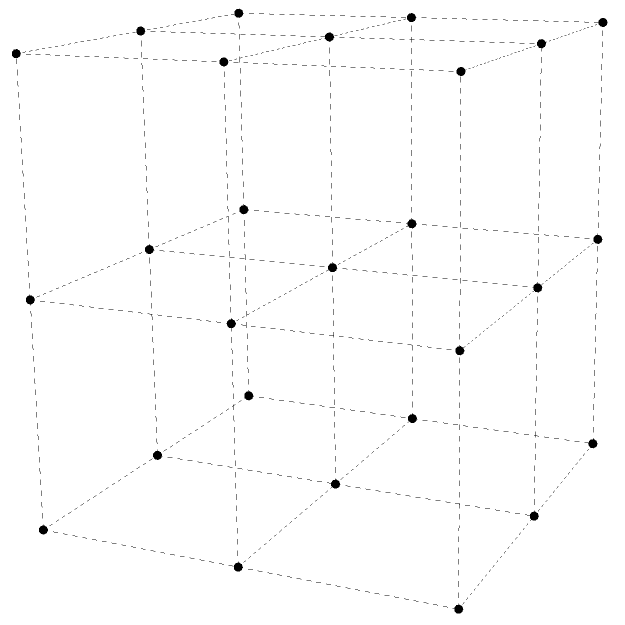
\includegraphics[width=0.25\textwidth]{Lattice.png}
    \caption{A cubic lattice.}
    \label{1F:cubicLattice}
\end{figure}\\
For the SH lattice in $D=4$, the fundamental region (the smallest $D$-dimensional polyhedron) is a $4$-dimensional hypercube, also called a tesseract.
This means that a SH lattice can be seen as a tassellation of the spacetime with tesseracts as elementary cells.
Each point of the lattice has $8$ nearest neighbours that are identified by the vectors obtained through all possible permutations of position and sign of $(\pm1,0,0,0)$.\\
The plaquette (the simplest bidimensional figure) is a square.
This will be important when implementing gauge theories on the lattice.
\begin{figure}[!htbp]
    \centering
    \hspace{0.1\textwidth}
    \begin{subfigure}[b]{0.25\textwidth}
        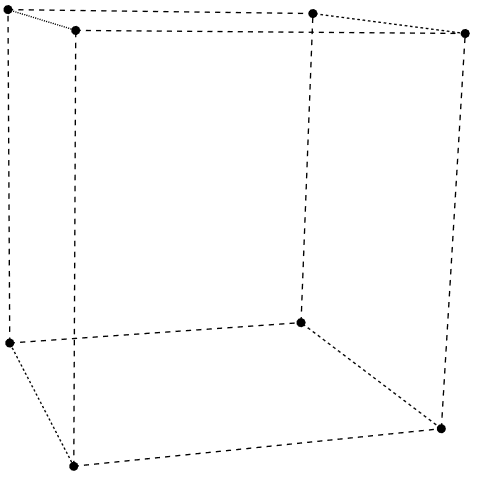
\includegraphics[width=\textwidth]{CubicCell.png}
        \caption{Simple cube.}
        \label{1F:CubicCell}
    \end{subfigure}
    \hspace{0.2\textwidth}
    \begin{subfigure}[b]{0.25\textwidth}
        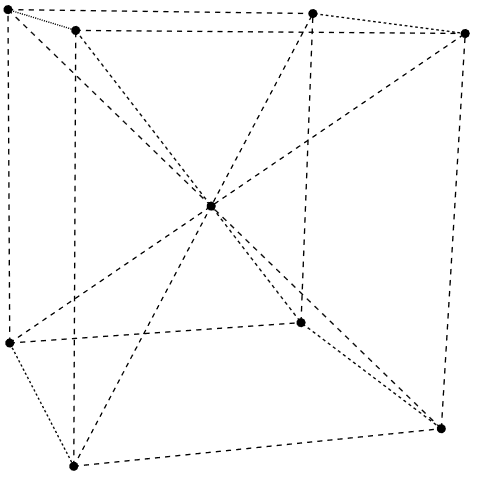
\includegraphics[width=\textwidth]{BodyCenteredCubicCell.png}
        \caption{Body-centered cube.}
        \label{1F:BCCubicCell}
    \end{subfigure}
    \hspace{0.2\textwidth}
    \caption{Tridimensional representation of a simple cubic cell (\ref{1F:CubicCell}) and a body-centered one (\ref{1F:BCCubicCell}).}
    \label{1F:ScBccCells}
\end{figure}

\subsubsection{Body-Centered Tesseract}
The SH lattice is not, of course, the only possible choice of a lattice in $4$ spacetime dimensions.
Another common choice, already used to simulate gauge theories~\cite{Celmaster:1982ht}, is the Body-Centered Tesseract (BCT).
It consists of packing the spacetime with tesseracts, as the name suggests, but considering both the corners and the centers of every hypercube as lattice sites.
Every site has, therefore, $24$ nearest neighbours: $16$ are identified by all possible sign permutations of $\pr{\pm\frac12,\pm\frac12,\pm\frac12,\pm\frac12}$, the $8$ remaining are the ones of the SH lattice.
The cell of this lattice is known as $24$-cell, shown in Figure \eqref{1F:24cell}, and the plaquettes are triangular.
\begin{figure}[!htbp]
    \centering
    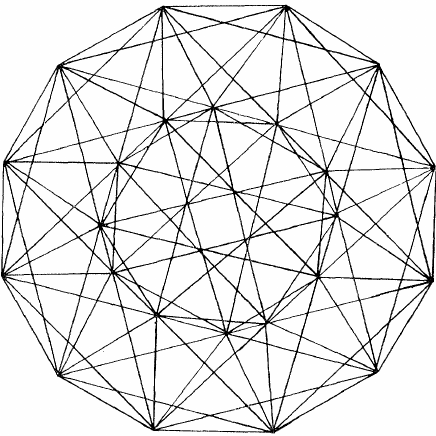
\includegraphics[width=0.33\textwidth]{24cell.png}
    \caption{Bidimensional projection of the $24$-cell.}
    \label{1F:24cell}
\end{figure}

\subsection{Scalar Fields on the Simple Hypercubic Lattice}
Let us consider a simple hypercubic lattice $\Lambda_{SH}$ extending over $L=L_1=L_2=L_3$ lattice spacings in the spatial directions and over $T=L_0$ lattice spacings in the temporal direction.
Let us also consider a scalar field $\phi(x)$, in order to introduce some useful tools that will be needed later.
As anticipated in the beginning of this section, a scalar field can only assume values on the sites of the lattice, therefore $x\in\Lambda_{SH}$, and let us assume, for simplicity, periodic boundary conditions on the fields, therefore $\phi(x+a\hat\mu L_\mu)=\phi(x)$.
The Fourier transform of the field becomes
\begin{equation}
    \tilde\phi(p)=\sum_x a^4 e^{-\i p\cdot x}\phi(x) \label{1:FourierScalar}
\end{equation}
and the allowed momenta are given by
\begin{equation}
    p_\mu=\frac{2\pi}{aL_\mu}n_\mu, \qquad n_\mu=0, \dots, L_\mu \label{1:Brillouin}
\end{equation}
This ensures that the momenta can take only the assigned values of the Brillouin zone \eqref{1:Brillouin} and therefore cannot go to infinity, providing a natural cutoff given by the lattice spacing $a$.\\
The discretization also implies that derivatives of the fields cannot be computed, therefore the lattice forward derivative is used:\footnote{Note that, in the continuum limit, the two derivatives coincide.}
\begin{equation}
    \partial_\mu\phi(x)\rightarrow \nabla_\mu\phi(x)=\frac{\phi(x+a\hat\mu)-\phi(x)}{a} \label{1:ForwardLatticeDerivative}
\end{equation}\\
Assuming a self-interaction potential $V(\phi)=\frac\lambda{4!}\phi^4$, the action \eqref{1:ActionScalar} can be written in terms of the lattice in the following way:
\begin{equation}
    S=a^4\sum_x\pr{\frac1{2a^2}\prs{\phi(x+a\hat\mu)-\phi(x)}^2+\frac12m^2\phi^2(x)+\frac\lambda{4!}\phi^4(x)} \label{1:ScalarActionLattice}
\end{equation}
A similar approach will be used in the following section to obtain the action for Yang-Mills theories.

\subsection{Gauge Fields on the Simple Hypercubic Lattice}
Let us now take into consideration a Yang-Mills theory, as in\secref{Sec:NonAbelianGaugeTheories}, with gauge group $\SUN$.
As anticipated before, gauge fields, being vector fields, can assume value only on links between sites of the lattice.\\
One could naively think that putting gauge vectors $A_\mu(x)$ on the links is enough, but this would explicitly break gauge invariance.
For this reason, Wilson's idea was to put the gauge group (and not algebra) elements, namely $U_\mu(x) = e^{\i a g A_\mu(x)}$, on the links.\\
The field $U_\mu(x)$ lives on the link connecting the site $x$ with the site $x+a\hat\mu$, therefore the link is oriented and link variables in negative directions can also be defined:\\
$U_{-\mu}(x) \equiv U^\dagger_\mu(x-a\hat\mu)$.
\begin{figure}[!htbp]
    \includegraphics[width=\textwidth]{linkVariables.png}
    \caption{Schematic visualization of link variables.}
    \label{1F:LinkVariables}
\end{figure}\\
Under a gauge transformation, the fields $U_\mu$ transform according to the following relation:
\begin{equation}
    U_\mu(x)\rightarrow \Omega(x) U_\mu(x) \Omega^\dagger(x+a\hat\mu) \label{1:GaugeTransformLinkVariable}
\end{equation}
where $\Omega(x)$ is any $\SUN$ matrix at the point $x$ on the lattice.
As a consequence of this relation, the trace of any product of links forming a closed path is a gauge-invariant quantity, thanks to the cyclic property of the trace.\\
With this in mind, Wilson's idea was to choose the simplest closed path possible: the plaquette, that in the simple hypercubic lattice is a square.
The product of link variables along a square plaquette is defined in the following way (the lattice spacing $a$ is set $=1$ for brevity of notation):
\begin{align*}
    U_{\mu\nu}(x) \equiv& U_\mu(x)U_\nu(x+\hat\mu)U_{-\mu}(x+\hat\mu+\hat\nu)U_{-\nu}(x+\hat\nu) =\\
    =& U_\mu(x)U_\nu(x+\hat\mu)U^\dagger_\mu(x+\hat\nu)U^\dagger_\nu(x) \numthis\label{1:Plaquette}
\end{align*}
Thus a gauge-invariant action, called Wilson action, can be written as follows:
\begin{equation}
    S_W[U]=\frac\beta{2N}\sum_{x\in\Lambda}\sum_{\mu<\nu}\Re\Tr[\id-U_{\mu\nu}(x)] \label{1:WilsonAction}
\end{equation}
where $\beta$ is a parameter that is going to be set in the following passages, $N$ the number of colors (the same $N$ in $\SUN$), the real part is needed to preserve unitarity and $U_{\mu\nu}$ is the plaquette of \eqref{1:Plaquette}.\\
\begin{figure}[!htbp]
\centering
    \begin{tikzpicture}
        \filldraw[black] (0,0) circle (3pt) node[anchor=north east]{$x$};
        \filldraw[black] (0,3) circle (3pt) node[anchor=south east]{$x+\hat\nu$};
        \filldraw[black] (3,0) circle (3pt) node[anchor=north west]{$x+\hat\mu$};
        \filldraw[black] (3,3) circle (3pt) node[anchor=south west]{$x+\hat\mu+\hat\nu$};
        \draw[ultra thick] (-0.5,0) -- (0,0);
        \draw[ultra thick] (0,-0.5) -- (0,0);
        \draw[ultra thick,->] (0,0) -- (1.5,0) node[anchor=north]{$U_\mu(x)$};
        \draw[ultra thick   ] (1.5,0) -- (3,0);
        \draw[ultra thick]  (3.5,0) -- (3,0);
        \draw[ultra thick] (3,-0.5) -- (3,0);
        \draw[ultra thick,->] (3,0) -- (3,1.5) node[anchor=west]{$U_\nu(x+\hat\mu)$};
        \draw[ultra thick   ] (3,1.5) -- (3,3);
        \draw[ultra thick]  (3.5,3) -- (3,3);
        \draw[ultra thick]  (3,3.5) -- (3,3);
        \draw[ultra thick,->] (3,3) -- (1.5,3) node[anchor=south]{$U^\dagger_\mu(x+\hat\nu)$};
        \draw[ultra thick   ] (1.5,3) -- (0,3);
        \draw[ultra thick] (-0.5,3) -- (0,3);
        \draw[ultra thick]  (0,3.5) -- (0,3);
        \draw[ultra thick,->] (0,3) -- (0,1.5) node[anchor=east]{$U^\dagger_\nu(x)$};
        \draw[ultra thick   ] (0,1.5) -- (0,0);
    \end{tikzpicture}
    \caption{Link variables building a plaquette $U_{\mu\nu}(x)$.}
    \label{1F:Plaquette}
\end{figure}\\
In the following part, the naive continuum limit is taken, showing that Wilson action reproduces Yang-Mills action of \eqref{1:YMActionEuclidean} when $a\to0$.
Let us start by defining an auxiliary field $B_\mu(x)$:
\begin{equation}
    B_\mu(x) = a g A^a_\mu(x)T^a \label{1:BField}
\end{equation}
thus the gauge group element becomes $U_\mu(x)=e^{\i B_\mu(x)}$.\\
The expansion for small $a$ of the plaquette $U_{\mu\nu}$ is:
\begin{align*}
    U_{\mu\nu} =& U_\mu(x)U_\nu(x+\hat\mu)U^\dagger_\mu(x+\hat\nu)U^\dagger_\nu(x) = \\
    =& e^{\i B_\mu(x)}e^{\i B_\nu(x+\hat\mu)}e^{-\i B_\mu(x+\hat\nu)}e^{-\i B_\nu(x)} = \\
    &\text{applying \eqref{1:ForwardLatticeDerivative}, } B_\mu(x+\hat\nu) = a\nabla_\nu B_\mu(x) \\
    =& e^{\i B_\mu(x)}e^{\i B_\nu(x)+a\nabla_\mu B_\nu(x)}e^{-\i B_\mu(x)-a\nabla_\nu B_\mu(x)}e^{-\i B_\nu(x)} \simeq \\
    &\text{From now on, the dependance from $x$ will be omitted.}\\
    &\text{Using BCH formula, } e^Xe^Y = e^{X+Y+\frac12\comm{X}{Y}}\text{, up to $O(a^2)$:} \\
    \simeq& \exp\Big\{\cancel{\i B_\mu} + \cancel{\i B_\nu} + \i a \nabla_\mu B_\nu - \cancel{\i B_\mu} - \i a \nabla_\nu B_\mu - \cancel{\i B_\nu}+\\
    &+\frac12\pr{-\comm{B_\mu}{B_\nu}+\cancel{\comm{B_\mu}{B_\nu}}+\cancel{\comm{B_\nu}{B_\mu}}-\comm{B_\mu}{B_\nu}}\Big\} = \\
    =& \exp{\i a\pr{\nabla_\mu B_\nu - \nabla_\nu B_\mu} - \comm{B_\mu}{B_\nu}}
\end{align*}
Now, substituting back \eqref{1:BField}, the discretized electromagnetic tensor can be found:
\begin{align*}
    U_{\mu\nu} \simeq& \exp{\i a^2 g \pr{\nabla_\mu \A_\nu - \nabla_\nu \A_\mu+ \i g \comm{\A_\mu}{\A_\nu}}} =  \exp{\i a^2 g \Fmunu} \simeq \\
    \simeq& \id + \i a^2 g \Fmunu - \frac12 a^4 g^2 \Fmunu F^{\mu\nu} + O(a^6) \numthis \label{1:PlaquetteSmalla}
\end{align*}
Finally, the small-$a$ approximation for the Wilson action \eqref{1:WilsonAction} can be obtained:
\begin{align*}
    S_W \simeq& \frac{\beta}{2N} \sum_{x\in\Lambda}\sum_{\mu<\nu} \Re\Tr(\cancel\id - \cancel\id - \i a^2 g \Fmunu^i T^i + \frac12a^4 g^2 \Fmunu^i F^{j\mu\nu}T^iT^j) = \\
    =& \underbrace{-i\frac{a^2\beta}{2N} \sum_{x\in\Lambda}\sum_{\mu<\nu} \Re(\Fmunu^i \Tr(T^i))}_{=0\text{ for \eqref{1:InfinitesimalSUN}}} + \frac{g^2a^4\beta}{4N} \sum_{x\in\Lambda}\sum_{\mu<\nu} \Re(\underbrace{\Fmunu^i F^{j\mu\nu}\Tr(T^iT^j)}_{=\frac12\Fmunu^i F^{i\mu\nu}\text{ for \eqref{1:NormCondSUN}}}) = \\
    =& \frac{g^2\beta}{8N} a^4\sum_{x,\mu,\nu}\Fmunu^i F^{i\mu\nu} \xrightarrow[a\to0]{} \frac{g^2\beta}{8N} \dV\Fmunu^i F^{i\mu\nu} \numthis \label{1:WilsonSmalla}
\end{align*}
where the Yang-Mills action \eqref{1:YMActionEuclidean} can be recognized if $\beta = \frac{2N}{g^2}$.

\subsubsection{Wilson Loops}
Now that the lattice action has been defined, observables need to be taken into account.
As mentioned below equation \eqref{1:GaugeTransformLinkVariable}, the trace of the product of link variables along any closed path is a gauge-invariant quantity.
This means that any quantity of the sort is a good candidate for an observable and, in fact, given any closed path $\gamma$ on the lattice, the Wilson loop is defined as follows:
\begin{equation}
    W[\gamma] \equiv \Tr\prs{\prod_{(x,\mu)\in\gamma}U_\mu(x)} \label{1:WilsonLoop}
\end{equation}
It is worthwile to mention that this definition is does not depend on the type of lattice and of boundary conditions chosen for such lattice.
If the path $\gamma$ does not include any temporal link, the loop is called \emph{spacelike Wilson loop}, otherwise it is called \emph{timelike Wilson loop}.
If all the links in $\gamma$ lie on the same plane, the Wilson loop is \emph{planar}, otherwise it is \emph{nonplanar}.
\begin{figure}[!htbp]
    \centering
    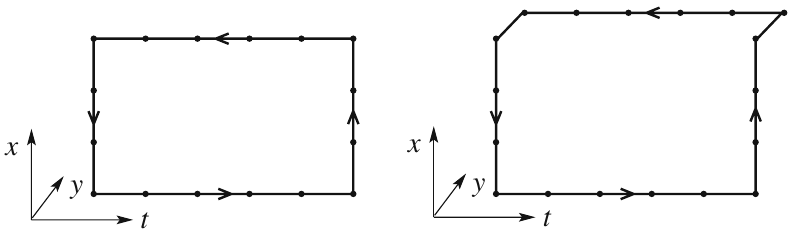
\includegraphics[width=0.8\textwidth]{WilsonLoops.png}
    \caption{Example of a planar (left) and nonplanar (right) Wilson loop.}
\end{figure}\\
Wilson loops are important for a variety of reasons, that will not be elaborated further as this is not the focus of this project, however it is worth knowing that they can be used as operators for purely gluonic bound states, the so-called \emph{glueballs}: the mass spectrum of these states can be obtained through the exponential decay of Wilson loops' correlation functions.

\subsubsection{Polyakov Loops}
Another important observable can be defined in lattices where periodic boundary conditions in the time direction are assumed.
Thanks to periodicity, a whole new class of closed paths arises: all paths that wind around the time direction.
A Polyakov loop is thus defined as a line at a fixed spatial position $\vec{x}=(x^1,x^2,x^3)$ that runs along the whole time direction:
\begin{equation}
    P(\vec{x}) \equiv \Tr\prs{\prod_{t=0}^{T-1} U_0(t,\vec{x})} \label{1:PolyakovLoop}
\end{equation}
The Polyakov loop has a lot of interesting properties: its physical interpretation is the world-line of a single static quark, therefore its expectation value is an order parameter of the deconfinement transition, as well as of a new global symmetry, called \emph{center symmetry}, arising from the periodicity of the time direction.\\
This means that, if the system is confined (quarks and gluons cannot move around freely), its expectation value is $0$, while if the system is deconfined, $\expval{P(\vec{x})}\neq0$.\\
Another property, that will be used in the simulations, is that the expectation value of the product of two Polyakov loops at distance $r=a\abs{\vec{x}-\vec{y}}$ is a function of the static quark-antiquark potential $V(r)$, as indicated below:
\begin{equation}
    \expval{P(\vec{x})P^\dagger(\vec{y})} \varpropto e^{-TaV(r)}\pr{1+O(e^{-Ta\Delta E})} \label{1:PolyakovPotential}
\end{equation}
where $\Delta E$ is the difference between $V(r)$ and the first excited energy level of the quark-antiquark pair.\\
The value of the potential $V(r)$ will be used, in this project, to study the recovery of rotational invariance when approaching the continuum limit.\\
Various methods of performing computer simulations of lattice field theory and how to obtain these quantities, such as plauette values, Wilson and Polyakov loops, is shown in the following chapter.


\newpage
\cleardoublepage
\pagestyle{myFancy}
\chapter{Computer Simulation of Pure Gauge Theories}
\section{Introduction}
Monte Carlo simulations are a powerful tool that can be used to evaluate observables in lattice field theory.
Given an observable $O$ (such as a plaquette, a Wilson or Polyakov loop, etc.), its vacuum expectation value is formally given by the functional integral
\begin{equation}
    \expval{O} = \frac1Z\int\DD[U]e^{-S[U]}O[U] \qquad \text{with} \qquad Z = \int\DD[U]e^{-S[U]}O[U] \label{2:Observable}
\end{equation}
where $\DD[U]$ is to be intended as a Haar measure.\\
This expression, however, cannot be evalued analytically except for very small lattices, therefore \eqref{2:Observable} is approximated by an average of the observable evaluated on $N$ sample gauge field configurations $\prc{U_n}$\footnote{Here the subscript $n$ distinguishes the different configurations.}, distributed according a probability density $\varpropto e^{-S[U_n]}$.\\
The expectation value is then obtained by computing the following sum for a sufficient number of configurations generated by the proper Monte Carlo algorithm(s):
\begin{equation}
    \expval{O} \simeq \frac1N\sum_{\prc{U_n}}O[U_n] \label{2:ExpValObs}
\end{equation}
Because of the probability density $\varpropto e^{-S[U_n]}$, only configurations $\prc{U_n}$ that minimize the action are \emph{good configurations}, as all other configurations are exponentially suppressed.
For this reason, generating totally random gauge fields on the lattice links is not an efficient way to evaluate \eqref{2:ExpValObs}, as most of the $\prc{U_n}$ will have a very small Boltzmann factor (the $e^{-S[U_n]}$) and expression \eqref{2:ExpValObs} will give incorrect results unless a huge number (orders of magnitude higher than what is reasonably possible) of different configurations is tried.\\
In order to avoid the evaluation of a great number of configurations that would contribute little-to-nothing to the observables' values, a sequence of configurations $\prc{U_n}$ is generated through a Markov chain process, built such that its stationary distribution minimizes the action $S[U]$. This process is usually called \emph{thermalization}.\\
Every process of this type must begin from a starting configuration, usually chosen by the user.
The main starting configurations are usually two: if the simulation begins with the fields in an ordered way (for example, all the gauge links set to the identity), the initial configuration is called \emph{cold start}, if the simulation begins with random gauge fields in every link, the initial configuration is called \emph{hot start}.
Of course, the Markov chain must have the same stationary distribution if the hot or cold start is chosen.\\
In this chapter the main Monte Carlo algorithms used to thermalize the starting configuration are presented, then the method for evaluating some observables of interest, such as plaquettes and Polyakov loops is explained.

\section{Markov Processes}
As anticipated before, a Markov chain is needed to evolve an arbitrary starting configuration $U_0$ up to a region of the configuration space with a relatively large Boltzmann factor $e^{-S}$, therefore with high probability.
A Markov process is charaterized by a probability of transitioning from a configuration $\alpha$ to another configuration $\beta$ depending only on $\alpha$ and $\beta$ and not on the history of the process, namely the previous transitions that already occourred.
In formulae, this is expressed as
\begin{equation}
    P(U_n=\beta|U_{n-1}=\alpha) = T(\beta|\alpha) \label{2:TransMatrix}
\end{equation}
That is to say that the transition matrix $T$ does not depend on the index $n$, representing the computer time.\\
Being a transition probability, the matrix $T$ must obey the following equations
\begin{align}
    0 \leq T(\beta|\alpha) \leq& 1 \qquad \forall \alpha,\beta \label{2:TPropProb} \\
    \sum_{\beta}T(\beta|\alpha) =& 1 \qquad \forall \alpha \label{2:TPropNorm}
\end{align}
where \eqref{2:TPropProb} is a consequence of $T(\beta|\alpha)$ representing a probability, and \eqref{2:TPropNorm} means that the probability of transitioning to any configuration must be $1$ (of course, the case when $\alpha=\beta$ is included as well).\\
In order for the stochastic process to not have any sink or source of probability, the following balance equation must be satisfied:
\begin{equation}
    \sum_\alpha T(\beta|\alpha)P(\alpha) = \sum_\alpha T(\alpha|\beta)P(\beta) \label{2:BalanceEq}
\end{equation}
This equation states that the probability of transitioning to the configuration $\beta$, written in the \lhs as the sum of the transition probability from the configuration $\alpha$ weighted by the probability $P(\alpha)$ that the system is actually in that configuration, must be equal to the probability of transitioning out of the configuration $\beta$, given by the probability of finding the system in the configuration $\beta$ times the transition probability $T(\alpha|\beta)$ over all the final configurations, in the right-hand side.
Thanks to \eqref{2:TPropNorm}, the \rhs is easily proven to be equal to $P(\beta)$.\\
A sufficient (but not necessary) condition to obey the balance equation \eqref{2:BalanceEq} is obtained by requiring that it holds true term-by-term, thus obtaining the detailed balance condition:
\begin{equation}
    T(\beta|\alpha)P(\alpha) = T(\alpha|\beta)P(\beta) \label{2:DetailedBalance}
\end{equation}
Although it is not a necessary condition, most algorithms, including the ones discussed in the following section, satisfy it.

\section{Monte Carlo Algorithms}
Monte Carlo algorithms are a class of algorithms that, singularly or combined together, allow to advance the Markov chain, while satisfying the condition presented in the previous section.
Each algorithm, if applied once, allows the transition from a configuration $U_{n-1}$ to a configuration $U_n$ (eventually the same as $U_{n-1}$). The repeated application of the algorithm allows to advance through the Markov chain.

\subsection{Metropolis Algorithm}
The first algorithm presented is the Metropolis algorithm. It is not very much efficient and usually it is not used in simulations, however it contains the fundamental steps that are present in some of the more advanced algorithms and it is quite easy to understand.
For this reasons it is ususally viewed as the \emph{``ancestor''} of all Monte Carlo algorithms and it is present in every textbook on the subject.\\
This algorithm consists in two steps that implement in one of the most simple ways the detailed balance condition \eqref{2:DetailedBalance}:
\begin{enumerate}[label=\arabic*)]
    \item A candidate configuration $\beta$ is chosen, according to some \emph{a priori} selection probability $T_0(\beta|\alpha)$, where $\alpha=U_{n-1}$.
    \item The candidate configuration $\beta$ is accepted as the new configuration $U_n$ with the acceptance probability
          \begin{equation}
              T_A(\beta|\alpha) = \min\pr{1,\frac{T_0(\alpha|\beta)\exp(-S[\beta])}{T_0(\beta|\alpha)\exp(-S[\alpha])}} \label{2:MetropolisAccProb}
          \end{equation}
          If it is not accepted, the unchanged configuration is considered again ($U_n=\alpha$) and the measurements are eventually made again.
\end{enumerate}
These two steps are repeated a sufficient amount of times up unitl the needed measurements are taken.\\
Note that the fact that $P(\alpha) = \frac{e^{-S[\alpha]}}{Z} \varpropto e^{-S[\alpha]}$ has been used.\\
The total transition probability $T$ is obtained through the product $T=T_0T_A$, as the two steps are independant from each other, and it is straightforward to see that it satisfies the detailed balance condition \eqref{2:DetailedBalance}:
\begin{align*}
    T(\beta|\alpha)P(\alpha) =& \frac1Z T_0(\beta|\alpha)T_A(\beta|\alpha)\exp(-S[\alpha]) = \\
    =& \frac1Z T_0(\beta|\alpha)\min\pr{1,\frac{T_0(\alpha|\beta)\exp(-S[\beta])}{T_0(\beta|\alpha)\exp(-S[\alpha])}}\exp(-S[\alpha]) = \\
    =& \frac1Z \min\pr{T_0(\beta|\alpha)\exp(-S[\alpha]), T_0(\alpha|\beta)\exp(-S[\beta])} = \\
    =& \frac1Z T(\alpha|\beta)\exp(-S[\beta]) = \\
    =& T(\alpha|\beta)P(\beta)
\end{align*}
\qed
In many cases a symmetric selection probability is used $T_0(\alpha|\beta)=T_0(\beta|\alpha)$, thus \eqref{2:MetropolisAccProb} simpliefies to:
\begin{equation}
    T_A(\beta|\alpha) = \min\pr{1, e^{-\Delta S}} \quad \text{with} \quad \Delta S = S[\beta]-S[\alpha] \label{2:MetropolisAccProbSymm}
\end{equation}
That means that if the new configuration lowers the action, the change is accepted with probability $1$ (as $e^{-\Delta S}>1$), otherwise it is accepted with a certain probability that decays exponentially as the difference in the action of the two configurations becomes greater.
This ensures that the algorithm \emph{moves across} the configuration space towards the minimums of the action, while allowing quantum fluctuations in order to not \emph{``get stuck''} on a local minimum.\\
If the change in the action is local (it involves a single link variable), $\Delta S$ can be computed using only the field values in the local neighbour. This will be the case for $\SUN$ gauge theories.

\subsubsection{Application to SU(N) Gauge Theories}
For a $\SUN$ gauge theory, the algorithm is implemented in the following way.
For each iteration, a single link is changed, then the acceptance probability is computed, a random number is extracted and, if it is less than the acceptance probability the change is accepted, otherwise it is rejceted. The algorithm is then iterated a certain number of times and measures are taken.\\
The candidate link $U'_\mu(x)$ for step 1 is generated in the vicinity of the old value $U_\mu(x)$, in order to not have a too great $\Delta S$ that would lead to too low accentance rates.
This can be done by exploiting the property that the product of any two elements of $\SUN$ is still an element of $\SUN$, therefore extracting a matrix $X\in\SUN$ near the identity allows to write the candidate link as:
\begin{equation}
    U'_\mu(x) = XU_\mu(x) \label{2:MetropolisCandidateLink}
\end{equation}
The matrix $X$ is chosen such that it has the same probability as $X^{-1}$, this way the selection probability $T_0$ is symmetric and the computation of the acceptance probability $T_A$ becomes easier.\\
For this reason, only the variation of the action $\Delta S$ must be computed, where of course the action is the Wilson action \eqref{1:WilsonAction}.
In particular, only the plaquettes containing the candidate link must be evaluated: the change in the action is local, so all the other plaquettes will have the same value both before and after the change of the link.
Hence $\Delta S = S[U'_\mu(x)]_{loc}-S[U_\mu(x)]_{loc}$.\\
In a SH lattice, each link is shared between $6$ plaquettes.
For each plaquette the change of the action is given by the change of the link, while the product of the other three gauge links, that is called \emph{staple} and will be indicated as $P_i$, remains unchanged.
Therefore, the local contribution to the action can be computed as:
\begin{equation*}
    S[U_\mu(x)]_{loc} = \frac\beta{2N} \sum_{i=1}^6 \Re\Tr\prs{\id-U_\mu(x)P_i} = \frac\beta{2N} \Re\Tr\prs{6\id-U_\mu(x)\sum_{i=1}^6P_i}
\end{equation*}
where the sum over all the staples is:
\begin{equation}
    A = \sum_{i=1}^6P_i = \sum_{\nu\neq\mu}\pr{U_\nu(x+\hat\mu)U^\dagger_\mu(x+\hat\nu)U^\dagger_\nu(x) + U^\dagger_\nu(x+\hat\mu)U^\dagger_\mu(x-\hat\nu)U_\nu(x-\hat\nu)} \label{2:SumOverStaples}
\end{equation}
The change of the action can now be computed as
\begin{equation}
    \Delta S = S[U'_\mu(x)]_{loc}-S[U_\mu(x)]_{loc} = \frac\beta{2N} \Re\Tr\prs{\pr{U_\mu(x)-U'_\mu(x)}A} \label{2:MetropolisActionVar}
\end{equation}
where $A$ is not affected by the change of $U_\mu(x)$.

\subsection{Heat Bath Algorithm}
The heat bath algorithm is an \emph{enhanced} version of the Metropolis algorithm, that combines the two steps into a single one and chooses the new candidate according to the probability distribution obtained by the computing the surrounding staples:
\begin{equation}
    \dd P(U) = \dd U \exp(\frac\beta{2N}\Re\Tr[U A]) \label{2:DistrProbHB}
\end{equation}
where $\dd U$ denotes the Haar integration measure of the gauge group and $A$ is computed according to \eqref{2:SumOverStaples}.
This probability distribution can be computationally quite demanding, but has the advantage that, unlike the Metropolis algorithm, the link variable always changes.\\
The implementation details depend on the gauge group, for this reason, the heat bath method for the gauge group $\SU(2)$ will be now explained\footnote{As matrixes of $\SUN$ can be built using $\SU(2)$ matrixes, the general case is just a little more complicated, but it follows the same principles.}.
Since the sum of any two $\SU(2)$ elements is proportional to another $\SU(2)$ element, the sum of all staples $A$ \eqref{2:SumOverStaples} can be written in the form
\begin{equation}
    A = V\sqrt{\det(A)} \qquad\text{with}\qquad V\in\SU(2) \label{2:SumOverStaplesSU2}
\end{equation}
where it can be proven that $\det(A)\geq0$.
Plugging into \eqref{2:DistrProbHB} and using the invariance of the Haar measure under trasformation of the origin of the group space ($\dd U = \dd (UV) = \dd X$), the distribution probability of the matrix $X=UV$ is
\begin{equation}
    \dd P(X) = \dd X \exp(\frac\beta{2N}\sqrt{\det(A)}\Re\Tr[X]) \label{2:DistrProbHBX}
\end{equation}
If a matrix $X$ distributed according to \eqref{2:DistrProbHBX} is generated, then the new candidate link, distributed according to \eqref{2:DistrProbHB}, is obtained as $U'_\mu(x) = XV^\dagger = \frac1{\sqrt{\det(A)}}XA^\dagger$.\\
Any $U\in\SU(2)$ matrix can be written in the following representation, using $4$ real numbers:
\begin{equation}
    U=x_0\id+\i \bm{x} \cdot \bm{\sigma} \qquad\text{with}\qquad \det(U)=\abs{x}^2=\sum_{i=0}^3x_i^2=1 \label{2:SU2Repr}
\end{equation}
where $\bm\sigma=\pr{\sigma_1,\sigma_2,\sigma_3}$ is a vector built using the Pauli matrices and $x=(x_0,\bm{x})$ can be seen as a normalized $4$-compnents vector.
Using this representation, the Haar measure in \eqref{2:DistrProbHBX} can be written as:
\begin{align*}
    \dd X =& \frac1{\pi^2} \dd^4x \delta\pr{x_0^2+\bm{x}-1} =\\
    =& \frac1{\pi^2} \dd^4x \frac{1}{2\sqrt{1-x_0^2}} \pr{\delta\pr{\abs{\bm{x}}-\sqrt{1-x_0^2}}+\delta\pr{\abs{\bm{x}}+\sqrt{1-x_0^2}}} \numthis\label{2:HaarMeasureHB}
\end{align*}
where a well known property of the Dirac delta function has been used.\\
The volume element can be rewritten in terms of the components of the vector $x$:
\begin{equation}
    \dd^4x = \dd x_0\dd\abs{x}\abs{x}^2\underbrace{\dd(\cos\theta)\dd\phi}_{\dd^2\Omega} \label{2:VolumeElemParam}
\end{equation}
Plugging back into \eqref{2:HaarMeasureHB} and integrating out the $\abs{\bm{x}}$ thanks to the delta functions (actually, only the first one contributes, as $x_i^2\leq1$ $\forall i$), the Haar measure takes the form:
\begin{equation}
    \dd X = \frac1{\pi^2}\dd x_0\dd^2\Omega\frac{1-x_0^2}{2\sqrt{1-x_0^2}} = \frac1{2\pi^2} \dd x_0 \dd^2\Omega \sqrt{1-x_0^2} \label{2:HaarMeasureHBSimplified}
\end{equation}
Then, in terms of the variables, the probability distribution becomes:
\begin{equation}
    \dd P(X) = \frac1{2\pi^2} \dd x_0 \dd\cos\theta \dd\phi \sqrt{1-x_0^2} \exp\pr{\frac\beta2 \sqrt{\det(A)}x_0} \label{2:DistrProbHBXSimplified}
\end{equation}
with $x_0\in[-1,1]$, $\cos\theta\in[-1,1]$, $\phi\in[0,2\pi)$, where $\Tr(X)=2x_0$ has been used.\\
Thus, the problem of generating a matrix $X$ distributed according to \eqref{2:DistrProbHBX} has been reduced to the determination of three random variables $x_0$, $\theta$, $\phi$, whose distribution factorizes, so they can be determined independetly from each other.
The random variable $x_0$, being distributed according to $\sqrt{1-x_0^2} \exp\pr{\frac\beta2 \sqrt{\det(A)}x_0}$, is determined through the auxiliary variable $\lambda\in[0,1]$ such that $x_0 = 1-2\lambda^2$, therefore
\begin{equation}
    \dd x_0\sqrt{1-x_0^2} \exp\pr{\frac\beta2 \sqrt{\det(A)}x_0} \varpropto \dd\lambda\lambda^2\sqrt{1-\lambda^2} \exp\pr{-\beta \sqrt{\det(A)}\lambda^2} \label{2:LambdaDistrHB}
\end{equation}
The variable $\lambda$ is generated with the polynomially modified Gaussian distribution density
\begin{equation}
    p_1(\lambda) = \lambda^2 e^{-\beta \sqrt{\det(A)}\lambda^2}
\end{equation}
and accepted with an accept/reject step using the square root function
\begin{equation}
    p_2(\lambda) = \sqrt{1-\lambda^2}
\end{equation}
There are several algorithms that can perform this computation in an efficient way~\cite{1998art, luscher1994portable}.\\
After this, the length $\abs{x} = \sqrt{1-x_0^2}$ is computed, in order to determine the remaining variables.\\
The variables $\cos\theta$ and $\phi$ are uniformely distributed, therefore a possible way of proceeding is by generating three random uniformely distributed numbers $r_1$, $r_2$ and $r_3$ in the interval $[-1,1)$ and accepting them only if $r_1^2+r_2^2+r_3^2\leq1$.
Then, the $3$-vector $(r_1,r_2,r_3)$ is normalized to length $\abs{x}$ computed before, obtaining $\bm{x} = (x_1,x_2,x_3)$.\\
After these steps, the vector $x=(x_0,\bm{x})$ can be used to generate the matrix $X$ according to \eqref{2:DistrProbHBX}, using representation \eqref{2:SU2Repr}, thus the new link variable can be obtained.\\
This algorithm rapidly leads the Markov process to a minimum of the action, however the risk of ``getting stuck'' on a local minimum is present.
For this reason, it is usually combined with the overrelaxation algorithm, discussed below.

\subsection{Overrelaxation Algorithm}

\section{Measurements}

\subsection{Plaquettes}

\subsection{Polyakov Loops}

\section{Brief Scheme of a Simulation}


\newpage
\cleardoublepage
\pagestyle{myFancy}
\chapter{Symmetries and Non-Hypercubic Lattices}

\section{Spacetime Symmetries Restoration}
The restoration of spacetime symmetries in the continuum limit is an important aspect of lattice field theory.
Minkowskian spacetime is invariant under the action of the Poincaré group, that includes translations, rotations in the $3$-dimensional space, and boosts.
When performing the Wick rotation, boosts become rotations in the planes formed by each one of the \emph{spacelike} axis and the euclidean time.
The euclidean spacetime is therefore invariant, in the continuum, under translations:
\begin{equation}
    x^\mu \to x^\mu + \varepsilon^\mu \label{3:TranslCont}
\end{equation}
and under rotations in $4$ dimensions:
\begin{equation}
    x^\mu \to R^\mu_\nu x^\nu \qquad\text{with}\qquad R\in\Orot(4) \label{3:RotCont}
\end{equation}
These invariances do not hold true anymore if the spacetime is discretized: a generic lattice is, in fact, invariant only under translations of multiples of the lattice spacing $a$:
\begin{equation}
    x \to x + a\mu \qquad\text{with}\qquad x\in\Lambda \label{3:TraslDiscr}
\end{equation}
and under certain rotations:
\begin{equation}
    x \to \Gamma x \qquad\text{with}\qquad x\in\Lambda, \Gamma\in G_\Lambda \label{3:RotDiscr}
\end{equation}
where $G_\Lambda\subset\Orot(4)$ is a discrete subset of the full rotational group $\Orot(4)$ that depends on the lattice $\Lambda$.
For example, $\Lambda=\Lambda_{SH}$ is a SH lattice, then $G_{\Lambda_{SH}}$ is the $384$-elements group with all possible reflections on every coordinate plane and rotations of multiples of $90^\degree$ around each one of the $4$ axis.\\
The fact that the symmetries between the discrete and the continuum cases are different is not a problem itself, as long as when approaching the continuum limit the lattice symmetries tend to the continuum ones.
This is the case for the translational symmetry: if $a\to0$, \eqref{3:TraslDiscr} becomes \eqref{3:TranslCont}.
However, the rotational symmetry is not restored when the continuum limit is taken (\eqref{3:RotDiscr} does not become \eqref{3:RotCont} when $a\to0$), as the Simple Hypercubic lattice is invariant under rotations of multiples of $90^\degree$ independently from the value of the lattice spacing.\\
For this reason, studies on the restoration of rotational symmetry have been made, through the computation of rotational invariant quantities.

\subsection{Rotational Invariance of the Static Quark Potential}
An example of these studies is the 1982 article of Lang and Rebbi~\cite{Lang:1982tj}, where the static quark potential $V(r)$, obtained from the correlator of two Polyakov loops (see \eqref{1:PolyakovPotential}), has been studied at different lattice spacings.
Through simulations of $\SU(2)$ lattice gauge theories the potential
\begin{equation}
    V(r) = -T\ln\expval{P^\dagger(r)P(0)} \label{3:LangRebbiPotential}
\end{equation}
has been obtained for different values of $r=(r_x, r_y, r_z)$ on lattices extending for $n_s$ lattice spacings in each of the space directions and $n_t$ lattice sites in the time direction.
Furthermore, the full gauge group $\SU(2)$ has been approximated by its discrete icosahedral subgroup $\tilde{Y}$ in order to improve the efficiency of the computation.
The varoius (about $1000$) potentials obtained for each site $r$ have then been fitted according to the expression
\begin{equation}
    V(r) = c_0 + c_1/r + c_2r \label{3:LangRebbiPotentialFit}
\end{equation}
Finally, a representation of the equipotential surfaces of expression \eqref{3:LangRebbiPotentialFit} has been plotted in Figure \eqref{3F:LangRebbi}.
\begin{figure}[!htbp]
    \centering
    \hfill
    \begin{subfigure}[b]{0.45\textwidth}
        \centering
        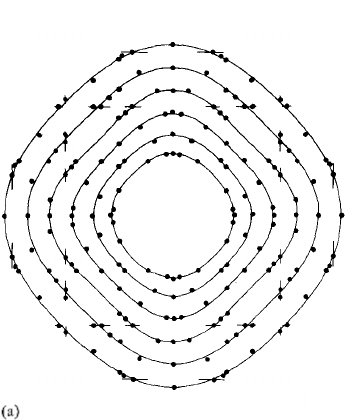
\includegraphics[width=0.857\textwidth]{LangRebbi_a.png}
        \caption{$\beta=2$, $n_s=8$, $n_t=4$.}
        \label{3F:LangRebbiA}
    \end{subfigure}
    \begin{subfigure}[b]{0.45\textwidth}
        \centering
        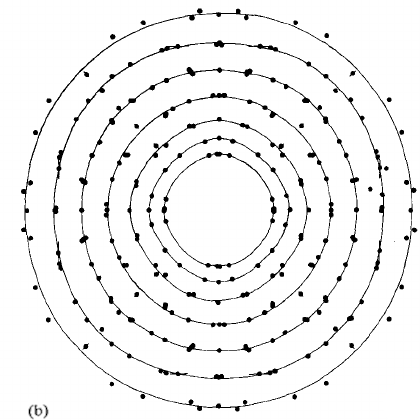
\includegraphics[width=\textwidth]{LangRebbi_b.png}
        \caption{$\beta=2.25$, $n_s=16$, $n_t=6$.}
        \label{3F:LangRebbiB}
    \end{subfigure}
    \hfill
    \caption{Representation of equipotential surfaces for larger (\ref{3F:LangRebbiA}) and smaller (\ref{3F:LangRebbiB}) lattice spacing.}
    \label{3F:LangRebbi}
\end{figure}\\
In Figure \eqref{3F:LangRebbiA} a lattice with $n_s=8$, $n_t=4$ and $\beta=\frac4{g^2}=2$ has been used, while Figure \eqref{3F:LangRebbiB} has been obtained with data from a lattice with $n_s=16$, $n_t=6$ and $\beta=2.25$.
As the lattice spacing depends, in first approximation, from $\beta$ in the following way:
\begin{equation}
    a(\beta) \approx e^{-\frac{12\pi^2}{11N^2}\beta} = e^{-\frac{3\pi^2}{11}\beta} \label{3:BetaLatticeSpacing} 
\end{equation}
the first plot corresponds to a higher value of $a$ than the second one\footnote{The rigorous determination of the lattice spacing is a rather compliacted matter that will not be explained further, as it is not the purpose of this project.}.\\
As can be easily seen, by lowering the lattice spacing equipotential surfaces tend to become circles, therefore the rotational invariance, that is broken in the lattice for any value of the lattice spacing, gets restored in the expectation value of the observables, making lattice field theory a \emph{``good''} theory capable of making meaningful predictions.

\section{Other Types of Lattice\label{Sec3:Lattices}}
In section\secref{Sec1:SHLattice} the Simple Hypercubic lattice has been defined.
Of course, it is not the only possible choice, although it is the simplest.
In fact, in order to further investigate the restoration of rotational symmetry and to make better predictions on rotational invariant quantities, other types of lattices have been used to simulate lattice field theories.

\subsection{Body-Centered Tesseract\label{Sec3:BCT}}
For example, the Body-Centered Tesseract (BCT) has been used for simulation of Yang-Mills theories.
It consists of packing the spacetime with tesseracts, as the name suggests, but considering both the corners and the centers of every hypercube as lattice sites (see Figure \eqref{3F:ScBccCells} for a tridimensional representation of a cubic cell \eqref{3F:CubicCell} and a body-centered cubic cell \eqref{3F:BCCubicCell}).\\
\begin{figure}[!htbp]
    \centering
    \hspace{0.1\textwidth}
    \begin{subfigure}[b]{0.25\textwidth}
        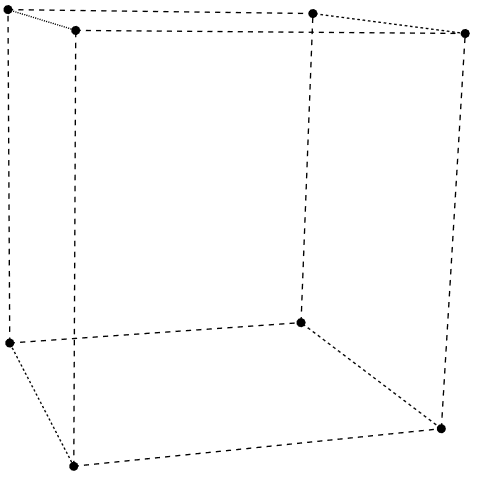
\includegraphics[width=\textwidth]{CubicCell.png}
        \caption{Simple cube.}
        \label{3F:CubicCell}
    \end{subfigure}
    \hspace{0.2\textwidth}
    \begin{subfigure}[b]{0.25\textwidth}
        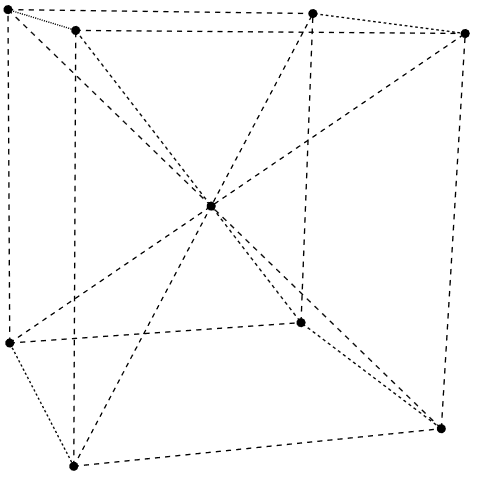
\includegraphics[width=\textwidth]{BodyCenteredCubicCell.png}
        \caption{Body-centered cube.}
        \label{3F:BCCubicCell}
    \end{subfigure}
    \hspace{0.2\textwidth}
    \caption{Tridimensional representation of a simple cubic cell (\ref{3F:CubicCell}) and a body-centered one (\ref{3F:BCCubicCell}).}
    \label{3F:ScBccCells}
\end{figure}\\
Every site of the BCT lattice has, therefore, $24$ nearest neighbours: $16$ are identified by all possible sign permutations of $\pr{\pm\frac12,\pm\frac12,\pm\frac12,\pm\frac12}$, the $8$ remaining are the ones of the SH lattice.
The cell of this lattice is known as $24$-cell, shown in Figure \eqref{3F:24cell}, and the plaquettes are triangular.
\begin{figure}[!htbp]
    \centering
    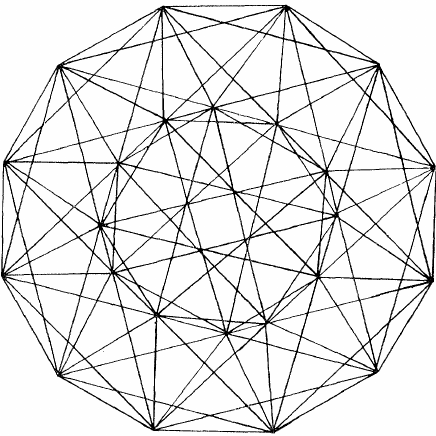
\includegraphics[width=0.33\textwidth]{24cell.png}
    \caption{Bidimensional projection of the $24$-cell.}
    \label{3F:24cell}
\end{figure}\\
This lattice has a $1152$-elements symmetry group $G_{\Lambda_{BCT}}$, allowing a lot more rotations and reflections than the $384$ of the SH lattice.

\subsection{\spFtext Coroots Lattice}
\spFtext is one of the five exceptional simple Lie groups, with Dynkin diagram \dynkin F4.
A more detailed explanation of exceptional Lie groups and algebras can be found in~\cite{adams1996lectures}.
Its root lattice is a $4$-dimensional body-centered hypercubic lattice, a BCT, while its dual, that is called the \spFtext coroots lattice, is the $4$-dimensional lattice with the symmetry group of highest order.
Each site of this lattice has $48$ nearest neighbours:
\begin{itemize}
    \item $24$ corresponding to the roots of \spFtext, individuated by all possible sign and position permutations of $(\pm1,\pm1,0,0)$;\
    \item $24$ corresponding to the coroots, the roots' dual vectors, individuated by\
    \begin{itemize}
        \item[$\circ$] the $8$ possible sign and coordinate permutations of $(\pm1,0,0,0)$\
        \item[$\circ$] the $16$ possible sign permutations of $\pr{\pm\frac12,\pm\frac12,\pm\frac12,\pm\frac12}$\
    \end{itemize}
\end{itemize}
This lattice is made up of two BCT lattices: the first one is the dual lattice, that is the same as\secref{Sec3:BCT}, the other is the root lattice, that is a BCT with lattice spacing $\sqrt2$ as can be seen as represented in Figure \eqref{3:F4cell}.
\begin{figure}[!htbp]
    \centering
    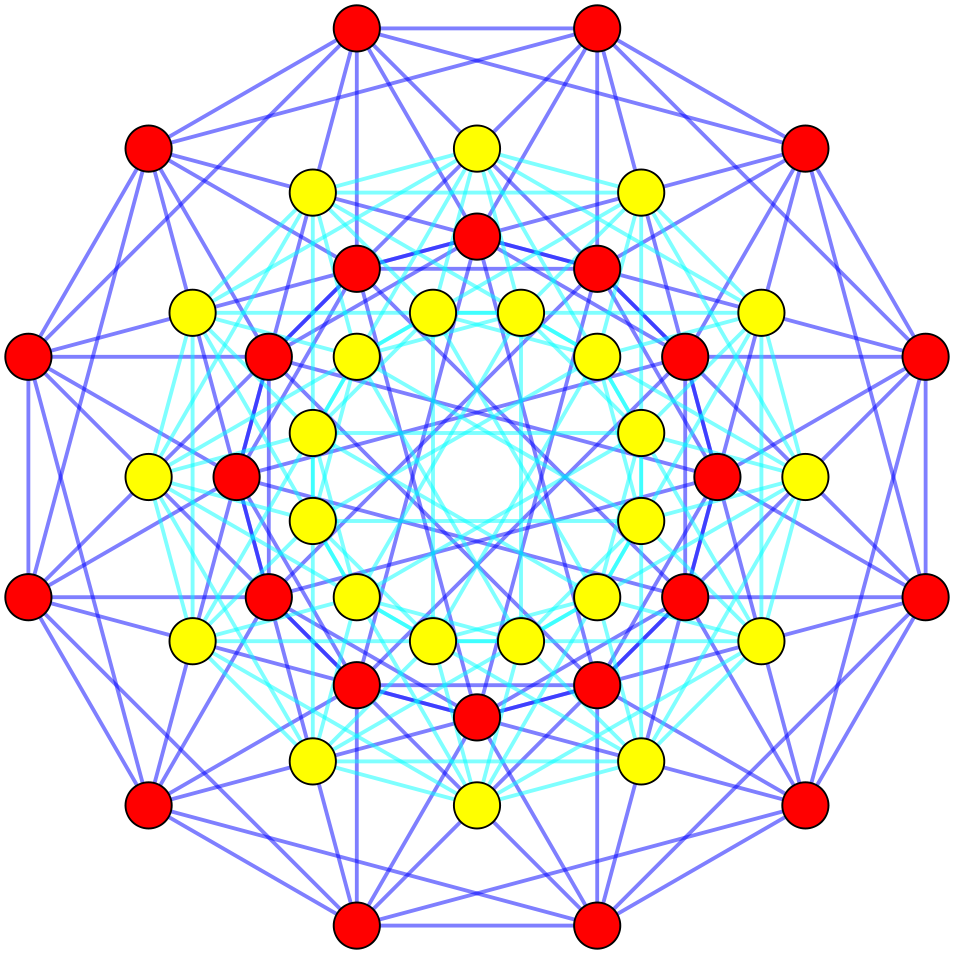
\includegraphics[width=0.33\textwidth]{F4_root_lattice.png}
    \caption{Bidimensional projection of the elementary cell of the \spFtext coroots lattice.\\
             The roots are represented in red and the coroots in yellow.}
    \label{3:F4cell}
\end{figure}\\
This lattice has a $2304$-elements symmetry group $G_{\Lambda_{\spF}}$, twice as the BCT symmetry group.

\section{Simulations on Higher Symmetric Lattices}
These lattices have been used, in literature, to perform Monte Carlo simulations of quantum field theories.

\subsection{Scalar Fields on \spFtext Lattice}
In~\cite{Neuberger:1987kt}, Neuberger presented the formulation of scalar fields in terms of the \spFtext lattice, where he discretized the action \eqref{1:ScalarActionEuclidean} assuming the simplest nearest neighbours interaction:
\begin{equation}
    S = \frac16\sum_{<xy>\in\Lambda}\pr{\phi(x)-\phi(y)}^2 +\sum_{x\in\Lambda}\pr{\frac12m^2\phi^2(x)+\frac\lambda4\phi^4(x)} \label{3:ScalarActionF4}
\end{equation}
where $<xy>$ indicates sum over nearest neighbours.\\
The Fourier transformation of the field $\phi(x)$ in the limit of infinte lattice volume is given by:
\begin{align*}
    \tilde\phi(k) =& \dV e^{\i k \cdot x} \phi(x) \\
    \phi(x) =& \frac1{2(2\pi)^4} \int\dd^4k e^{-\i k \cdot x} \tilde\phi(k)
\end{align*}
and the kinetic energy of \eqref{3:ScalarActionF4} at infinite volume is:
\begin{align*}
    \text{K.E.} =& \frac1{6(2\pi)^4} \int\dd^4k \abs{\tilde\phi(k)}^2\pr{\sum_\mu\pr{1-\cos(k_\mu)} +\sum_\pm\pr{1-\cos(\frac{k_1\pm k_2\pm k_3\pm k_4}{2})}} =\\
    =& \dots = \frac{1}{12(2\pi)^4} \int\dd^4k \abs{\tilde\phi(k)}^2\pr{k^2-\frac{1}{72}k^4+O(k^6)} \numthis\label{3:ScalarKE}
\end{align*}
The fact that the fourth order term is proportional to the square of the second order one is a feature of all symmetry-preserving lattice actions.\\
This work lead to some analytical~\cite{Bhanot:1990zd} and numerical~\cite{Bhanot:1990ai} results and to an upper bound prediction for the mass of the Higgs boson~\cite{Heller:1990sg} more than $20$ years before its actual discovery.

\subsection{Gauge Theories on BCT Lattice}
In~\cite{Celmaster:1982ht}, Celmaster presented the first computations for an $\SU(2)$ theory on a BCT.
Being a different lattice, where the plaquette is a triangle and not a square, a new action has to be defined: one that is invariant under the BCT group, with the correct classical continuum limit is:
\begin{equation}
    S_{BCT} = \frac1{2g^2} \sum_\bigtriangleup \Re\Tr \Utriang = \frac\beta8 \sum_\bigtriangleup \Re\Tr \Utriang \label{3:BCTAction}
\end{equation}
where $\Utriang$ is the triangular plaquette, defined as
\begin{equation}
    \Utriang = U_v(x)U_w(x+\hat{v})U_{-v-w}(x+\hat{v}+\hat{w}) = U_v(x)U_w(x+\hat{v})U^\dagger_{v+w}(x) \label{3:PlaqTriang}
\end{equation}
where $v$ and $w$ are labels indicating the possible nearest-neighbours directions, described in\secref{Sec3:BCT}, such that $v+w$ is a valid direction.
\begin{comment}
\begin{figure}[!hbtp]
    \centering
    \begin{tikzpicture}
        \filldraw[black]  (0,0) circle (3pt) node[anchor=north east]{$x$};
        \filldraw[black]  (2,0) circle (3pt) node[anchor=north west]{$x+\hat{v}$};
        \filldraw[black]  (1,1.732) circle (3pt) node[anchor=south]{$x+\hat{v}+\hat{w}$};
        \draw[ultra thick,->] (0,0) -- (1,0) node[anchor=north]{$U_v(x)$};
        \draw[ultra thick   ] (1,0) -- (2,0);
        \draw[ultra thick,->] (2,0) -- (1.5,0.866) node[anchor=south west]{$U_w(x+\hat{v})$};
        \draw[ultra thick   ] (1.5,0.866) -- (1,1.732);
        \draw[ultra thick,->] (1,1.732) -- (0.5,0.866) node[anchor=south east]{$U^\dagger_{v+w}(x)$};
        \draw[ultra thick   ] (0.5,0.866) -- (0,0);
    \end{tikzpicture}
    \caption{Schematization of an elementary triangular plaquette.}
    \label{3F:PlaqTriang}
\end{figure}\\
\end{comment}
\begin{figure}[!hbtp]
    \centering
    \begin{tikzpicture}
        \filldraw[black]  (0,0) circle (3pt) node[anchor=north east]{$x$};
        \filldraw[black]  (3,0) circle (3pt) node[anchor=north west]{$x+\hat{v}$};
        \filldraw[black]  (1.5,2.598) circle (3pt) node[anchor=south]{$x+\hat{v}+\hat{w}$};
        \draw[ultra thick,->] (0,0) -- (1.5,0) node[anchor=north]{$U_v(x)$};
        \draw[ultra thick   ] (1.5,0) -- (3,0);
        \draw[ultra thick,->] (3,0) -- (2.25,1.299) node[anchor=south west]{$U_w(x+\hat{v})$};
        \draw[ultra thick   ] (2.25,1.299) -- (1.5,2.598);
        \draw[ultra thick,->] (1.5,2.598) -- (0.75,1.299) node[anchor=south east]{$U^\dagger_{v+w}(x)$};
        \draw[ultra thick   ] (0.75,1.299) -- (0,0);
    \end{tikzpicture}
    \caption{Schematization of an elementary triangular plaquette.}
    \label{3F:PlaqTriang}
\end{figure}\\
For example, if $v=(+1,0,0,0)$ and $w=(0,+1,0,0)$, then they add up to $v+w=(+1,+1,0,0)$, that is not one of the nearest-neighbours vectors, whereas $v=(+1,0,0,0)$ and $w=\pr{-\frac12,+\frac12,-\frac12,+\frac12}$ add up to $v+w=\pr{+\frac12,+\frac12,-\frac12,+\frac12}$, that is a valid direction.
In Figure \eqref{3F:PlaqTriang} an example of an elementary triangular plaquette is shown.\\
There are $96$ such triangles touching each site and each edge is shared between $8$ triangles.
By comparison, on the SH lattice there are $24$ elementary square plaquettes touching each site and each edge is contiguous to $6$ squares.\\
In~\cite{Celmaster:1983hs} and~\cite{Celmaster:1983vy} Celmaster presented the first simulation results for the $\SU(2)$ gauge theory on the BCT lattice, explaining the algorithm used for the simulations in \cite{CELMASTER1985415}.

\subsubsection{Average Plaquette Value on BCT}
In~\cite{Celmaster:1983vy} a study on the average value of the plaquette is presented: it is plotted \wrt $\beta$ in Figure \eqref{3F:AvgPlaqBCTSH}.\\
As can be seen, the BCT average plaquette better follows the strong and weak coupling expansions, that are analytical approximations valid, respectively, for $\beta\to0$ ($\Leftrightarrow g\to\infty$) and for $\beta\to\infty$ ($\Leftrightarrow g\to0$).
\begin{figure}[!htbp]
    \centering
    \begin{subfigure}[b]{0.475\textwidth}
        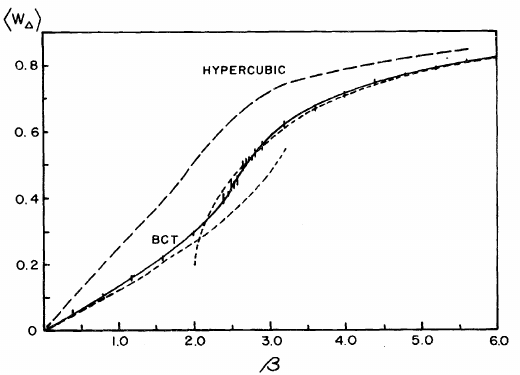
\includegraphics[width=\textwidth]{AvgPlaq1.png}
        \caption{Comparison between $\expval{W_\bigtriangleup}$ on BCT and SH lattices. The short-dashed lines represent weak and strong coupling expansions.}
        \label{3F:AvgPlaqBCTSH}
    \end{subfigure}
    \hfill
    \begin{subfigure}[b]{0.475\textwidth}
        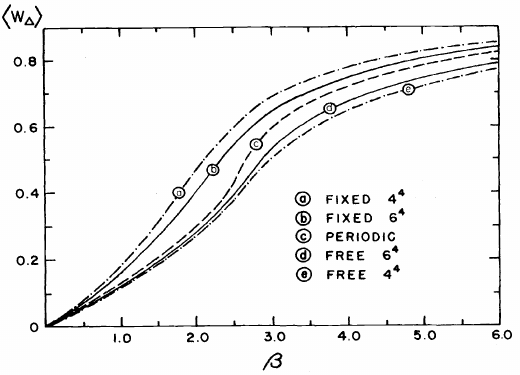
\includegraphics[width=\textwidth]{AvgPlaq2.png}
        \caption{Dependence of $\expval{W_\bigtriangleup}$ on boundary conditions in different BCT lattices, with different boundary conditions.}
        \label{3F:AvgPlaqBoundary}
    \end{subfigure}
    \caption{Average value of the plaquette $\expval{W_\bigtriangleup}$ on a BCT lattice as a function of $\beta$.}
\end{figure}\\
In the same article the influence of the boundary conditions on the average value of the plaquette is also investigated.
Three different boundary conditions are simulated: periodic, that means that lattice has the topology of a $4$-dimensional torus, free, that means that links on the boundary are free to assume any $\SU(2)$ value, and fixed, that means that links on the boundary are constrained to assume a certain $\SU(2)$ value.
The results are plotted in Figure \eqref{3F:AvgPlaqBoundary}.\\
From the plot, it can be seen that $\expval{W_\bigtriangleup}_{free} \leq \expval{W_\bigtriangleup}_{periodic} \leq \expval{W_\bigtriangleup}_{fixed}$, which is an inequality discussed by Mütter and Schilling in~\cite{Konig:1983dg}.\\
It is also pointed out that computer runtime of BCT simulations was slower by a factor of approximately $2.5$ than SH simulations, but this is compensated by having $3$ times as many degrees of freedom, that become $\frac{11}{3}$ as many if a gauge fixing is done, and $\frac{16}{3}$ as many plaquettes for each site.
Furthermore, having $12$ symmetry axes instead of $4$ provides a higher symmetry of the observables allowing for better checks on computations.

\subsubsection{String Tension}
In~\cite{Celmaster:1983hs} the $\SU(2)$ string tension is obtained from measurements of ratios of Wilson loops on a $6^4$ BCT lattice.\\
On a BCT lattice, there are two types of Wilson loops:
\begin{itemize}
    \item Rectangular Wilson loops $W_R(n,m)=\frac12\expval{\Tr U_R(n,m)}$\
    \item Triangular Wilson loops $W_T(n)=\frac12\expval{\Tr U_T(n)}$
\end{itemize}
where $U_R(n,m)$ is the product of link variables over an $n\times m$ rectangle and $U_T(n)$ is the product of link variables over an equilateral triangle of side $n$.\\
Assuming that Wilson loops are fitted by:
\begin{equation}
    W = e^{-\sigma A -b(\text{perimeter}) +\text{const.}} \label{3:WilsonFit}
\end{equation}
where $A$ is the area of the loop, then the string tension $\sigma$ can be obtained through logarithmic ratios:
\begin{align}
    \chi(2) =& -\ln(\frac{W_R(1,1)W_R(2,2)}{W_R^2(1,2)}) \\
    R_T(3) =& -\frac{2}{\sqrt3}\ln(\frac{W_T(1)W_T(3)}{W_T^2(2)})
\end{align}
Results of the simulations are plotted in Figure \eqref{3F:LogLoopRatios}, assuming no correlations between loop fluctuations in the computation of the error bars.
\begin{figure}[!htbp]
    \centering
    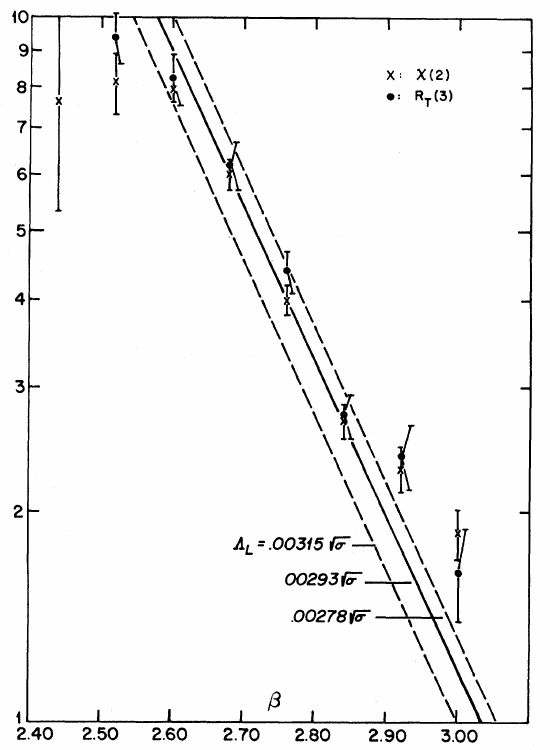
\includegraphics[width=0.4\textwidth]{LogarithmicRatios.png}
    \caption{$\SU(2)$ logarithmic loop ratios as a function of $\beta$ on a $6^4$ BCT lattice.}
    \label{3F:LogLoopRatios}
\end{figure}\\
The logarithmic loop ratio $\chi(2)$ agrees with the asymptotic freedom curve in the region $2.68\leq\beta\leq2.84$ far better than any other result obtained with simulations on SH lattices.
This is a consequence of the fact that the BCT action has smaller $O(a^2)$ corrections than usual at small $\beta$, therefore finite-spacing corrections are smaller for this action than for others previously examined.
Therefore, BCT lattices with less sites than SH lattices could be used to obtain data with the same accuracy, at a given lattice spacing $a$.
In the article is stated that, if the lattice spacing is sent $a\to a/2$, a SH lattice would require $16$ times as more sites in order to keep the physical size of the Wilson loop constant, while if the same operation is done on a BCT lattice, the increment in the number of sites would be much less, using about $16$ times less CPU time than the Wilson action.\\
Furthermore, $R_T(3)$ is compatible with $\chi(2)$ within error bars: this is a confirmation of the area-law dependence of equation \eqref{3:WilsonFit}.\\
In conclusion, simulations on BCT lattices provide better results, with more rotational invariance than those on other lattices, at a cost of a slightly higher computational time.


\newpage
\cleardoublepage
\pagestyle{myFancy}
\chapter{Simulation Results\label{Chap:SimulationResults}}
In this chapter original results from simulations are presented.
The code used to perform such simulations is based on the code originally developed for the calculations presented in refs.~\cite{Panero:2009tv,Mykkanen:2012ri}.

\section{Rotational Invariance Restoration}
This first section has the aim to reproduce the rotational invariance restoration of ref.~\cite{Lang:1982tj} for the continuous group $\SU(2)$ (and not for its discrete icosahedral subgroup $\tilde{Y}$, like explained in \secref{Sec3:RotInv}).\\
This is done by evaluating the correlator of two Polyakov loops as discussed in \secref{Sec2:PolyakovLoops}, computed on two different lattices with two different values of $\beta$, corresponding to two different lattice spacings.

\subsection{Setup of the Simulations}
The lattices are taken to be periodic in every direction, with $n_s$ sites in each spatial direction ($n_s=n_x=n_y=n_z$) and $n_t$ sites in the time direction.
The lattice has, therefore, $n_s^3n_t$ sites.\\
The simulations are run starting from a cold configuration, with $2500$ thermalization steps, where each Monte Carlo step is composed of one heat-bath step followed by three overrelaxation steps.
While the plaquette is observed to thermalize very quickly, after $O(10)$ steps in preliminary simulations with both hot and cold starts, we estimate $2500$ thermalization steps to be enough to ensure full thermalization of the configurations.\\
After thermalization, $20000$ measurements are taken of every possible independent correlator between two Polyakov loops, with $2$ updates between each measurement.\\
On a lattice with $n_s$ spatial sites in each direction, only pairs of Polyakov loops whose distance, in each spatial direction, is less than or equal to $n_s/2$ are independent: for example a pair of Polyakov loops extending for $n_s/2+1$ sites in a certain direction is equivalent to the Hermitian conjugate of a couple extending for $n_s/2-1$ sites, because of the periodic boundary conditions (see \eqref{2:nonzeroMomPolyakov}).
But, since the Polyakov loop correlator expectation value is real, they have the same numerical value.\\
\figref{4F:PolyakovPeriodic} represents a graphical visualization of this fact.
\begin{figure}[!htbp]
    \centering
    \begin{subfigure}[b]{0.48\textwidth}
        \centering
        \begin{tikzpicture}
            \draw[step=1.0,dotted] (0,0) grid (6,4);
            \draw[->] (0,0) -- (1,0) node[anchor=north west]{$x$};
            \draw[->] (0,0) -- (0,1) node[anchor=south east]{$t$};
            
            \draw (5,0) node[anchor=south west]{$P(x)$};
            \draw[thick,->] (5,0) -- (5,1);
            \draw[thick,->] (5,1) -- (5,2);
            \draw[thick,->] (5,2) -- (5,3);
            \draw[thick,->] (5,3) -- (5,4);
            
            \draw (3,4) node[anchor=north east]{$P^\dagger\pr{x+\frac{n_s}{2}+1}$};
            \draw[thick,->] (3,4) -- (3,3);
            \draw[thick,->] (3,3) -- (3,2);
            \draw[thick,->] (3,2) -- (3,1);
            \draw[thick,->] (3,1) -- (3,0);
            
            \draw[very thick,red] (5,2) -- (6,2);
            \draw[very thick,red] (1.5,2) node[anchor=south]{$n_s/2+1$};
            \draw[very thick,red,->] (0,2) -- (3,2);
        \end{tikzpicture}
    \end{subfigure}
    \hfill
    \begin{subfigure}[b]{0.48\textwidth}
        \centering
        \begin{tikzpicture}
            \draw[step=1.0,dotted] (0,0) grid (6,4);
            \draw[->] (0,0) -- (1,0) node[anchor=north west]{$x$};
            \draw[->] (0,0) -- (0,1) node[anchor=south east]{$t$};
            
            \draw (5,0) node[anchor=south west]{$P^\dagger(x)$};
            \draw[thick,->] (5,4) -- (5,3);
            \draw[thick,->] (5,3) -- (5,2);
            \draw[thick,->] (5,2) -- (5,1);
            \draw[thick,->] (5,1) -- (5,0);
            
            \draw (3,4) node[anchor=north east]{$P\pr{x-\pr{\frac{n_s}{2}-1}}$};
            \draw[thick,->] (3,0) -- (3,1);
            \draw[thick,->] (3,1) -- (3,2);
            \draw[thick,->] (3,2) -- (3,3);
            \draw[thick,->] (3,3) -- (3,4);
            
            \draw[very thick,red,->] (3,2) -- (5,2);
            \draw[very thick,red] (4,2) node[anchor=south]{$n_s/2-1$};
        \end{tikzpicture}
    \end{subfigure}
    \caption{The correlator of two Polyakov loops separated by $n_s/2+1$ sites (left) is equal to the Hermitian conjugate of the correlator of two Polyakov loops at a distance of $n_s/2-1$ sites (right), \ie $\expval{P(x)P^\dagger\pr{x+\frac{n_s}{2}+1}}=\expval{P\pr{x-\pr{\frac{n_s}{2}-1}}P^\dagger(x)}^\dagger$.}
    \label{4F:PolyakovPeriodic}
\end{figure}\\
Therefore, we only consider correlators of pairs of Polyakov loops whose spatial separations are given by the lattice vectors lying within a cube of size $n_s$ having the origin $(0,0,0)$ as a vertex.
Correlators associated with the same separation vector are then averaged together, to increase statistics.
%and the uncorrelated empirical standard deviation is computed as an estimate of the error.

\subsection{Analysis of Data}
After checking that each correlator's mean value is real (the imaginary part necessarily has to be compatible with $0$ within machine precision), these averages are used to compute the potential, in units of the inverse of the lattice spacing $a$, as:
\begin{equation}
    V(x,y,z) = -\frac{1}{n_t}\ln\expval{P(0)P^\dagger(x,y,z)} \label{4:Potential}
\end{equation}
where $(x,y,z)\in\prc{(0,0,0),\dots,\pr{\frac{n_s}{2},\frac{n_s}{2},\frac{n_s}{2}}}$.
The standard deviation is computed with the usual error propagation formula.\\
Plots like \figref{3F:LangRebbi} are obtained considering a section of the lattices used, specifically the $xy$-plane, that is done by plotting only values of $V(x,y,z=0)$.\\
In order to verify that there are no anisotropies, all the three main coordinate planes are plotted in \figref{4F:PotentialPlanes}.\\
The values obtained for corresponding points in each plane are compatible with each other within their statistical uncertainties and there is no visible difference between different coordinate planes.
This justifies choosing arbitrarily one plane for each lattice.
\begin{figure}[!htbp]
    \centering
    \begin{subfigure}[t]{\textwidth}
        \centering
        \begin{subfigure}[t]{0.32\textwidth}
            \renewcommand\thesubfigure{\alph{subfigure}1}
            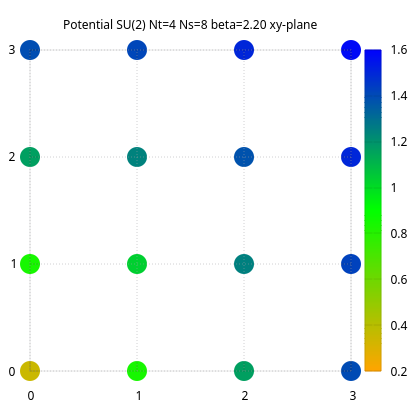
\includegraphics[width=\textwidth]{nt4_ns8_beta2.20/xy.png}
            \caption{$xy$-plane}
            \label{4F:PotentialPlanes48xy}
        \end{subfigure}
        \hfill
        \begin{subfigure}[t]{0.32\textwidth}
            \addtocounter{subfigure}{-1}
            \renewcommand\thesubfigure{\alph{subfigure}2}
            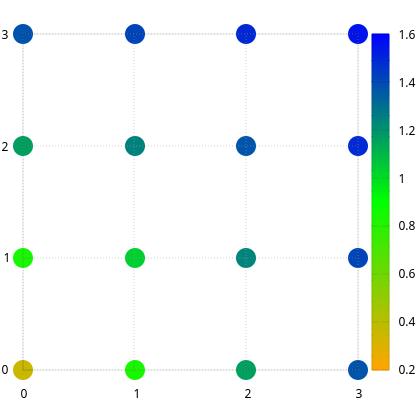
\includegraphics[width=\textwidth]{nt4_ns8_beta2.20/xz.png}
            \caption{$xz$-plane}
            \label{4F:PotentialPlanes48xz}
        \end{subfigure}
        \hfill
        \begin{subfigure}[t]{0.32\textwidth}
            \addtocounter{subfigure}{-1}
            \renewcommand\thesubfigure{\alph{subfigure}3}
            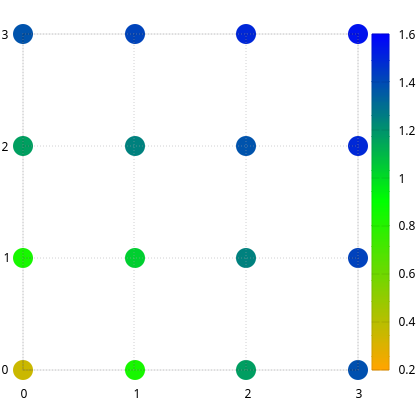
\includegraphics[width=\textwidth]{nt4_ns8_beta2.20/yz.png}
            \caption{$yz$-plane}
            \label{4F:PotentialPlanes48yz}
        \end{subfigure}
        \addtocounter{subfigure}{-1}
        \caption{Lattice with $n_t=4$, $n_s=8$, $\beta=2.20$.}
        \label{4F:PotentialPlanes48}
    \end{subfigure}\\
    \vspace{\baselineskip}
    \begin{subfigure}[b]{\textwidth}
        \centering
        \begin{subfigure}[b]{0.32\textwidth}
            \renewcommand\thesubfigure{\alph{subfigure}1}
            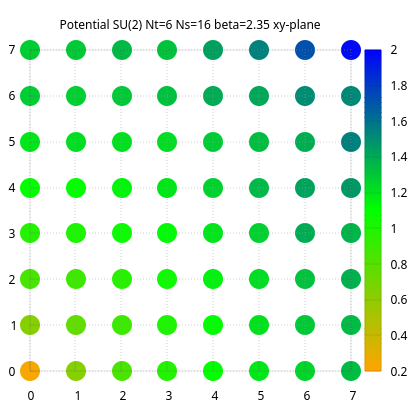
\includegraphics[width=\textwidth]{nt6_ns16_beta2.35/xy.png}
            \caption{$xy$-plane}
            \label{4F:PotentialPlanes616xy}
        \end{subfigure}
        \hfill
        \begin{subfigure}[b]{0.32\textwidth}
            \addtocounter{subfigure}{-1}
            \renewcommand\thesubfigure{\alph{subfigure}2}
            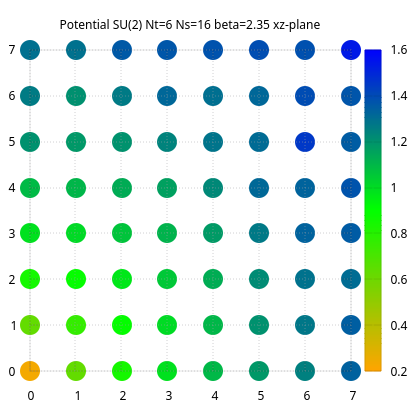
\includegraphics[width=\textwidth]{nt6_ns16_beta2.35/xz.png}
            \caption{$xz$-plane}
            \label{4F:PotentialPlanes616xz}
        \end{subfigure}
        \hfill
        \begin{subfigure}[b]{0.32\textwidth}
            \addtocounter{subfigure}{-1}
            \renewcommand\thesubfigure{\alph{subfigure}3}
            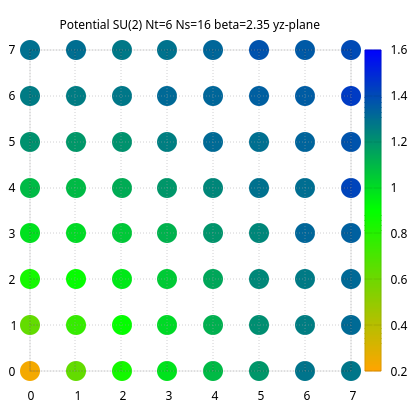
\includegraphics[width=\textwidth]{nt6_ns16_beta2.35/yz.png}
            \caption{$yz$-plane}
            \label{4F:PotentialPlanes616yz}
        \end{subfigure}
        \addtocounter{subfigure}{-1}
        \caption{Lattice with $n_t=6$, $n_s=16$, $\beta=2.35$.}
        \label{4F:PotentialPlanes616}
    \end{subfigure}
    \caption{Plots of the static quark potential in the three coordinate planes for two different lattices. The colored scale represent the potential in lattice spacing units.}
    \label{4F:PotentialPlanes}
\end{figure}
\begin{figure}[!htbp]
    \centering
    \begin{subfigure}[b]{0.48\textwidth}
        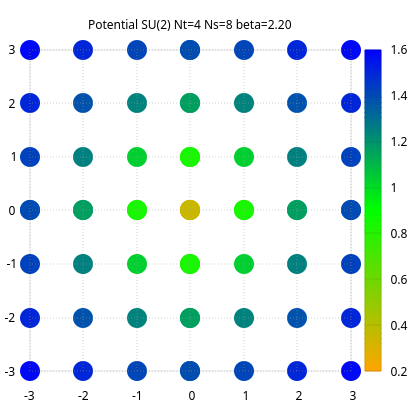
\includegraphics[width=\textwidth]{nt4_ns8_beta2.20/RotSymm.png}
        \caption{Lattice with $n_t=4$, $n_s=8$, $\beta=2.20$.}
        \label{4F:PotentialRestorationLargea}
    \end{subfigure}
    \begin{subfigure}[b]{0.48\textwidth}
        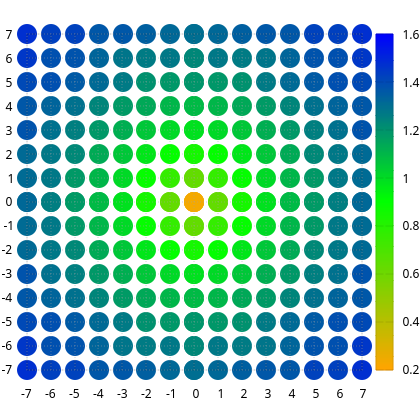
\includegraphics[width=\textwidth]{nt6_ns16_beta2.35/RotSymm.png}
        \caption{Lattice with $n_t=6$, $n_s=16$, $\beta=2.35$.}
        \label{4F:PotentialRestorationSmalla}
    \end{subfigure}
    \caption{Rotational invariance restoration of the static quark potential.}
    \label{4F:PotentialRestoration}
\end{figure}\\
In order to give a more ``complete'' view, the data from \figref{4F:PotentialPlanes48xy} and \figref{4F:PotentialPlanes616xy} are reflected relative to the $x$ and $y$ axes, obtaining the plots in \figref{4F:PotentialRestoration}.\\
In both \figref{4F:PotentialPlanes} and \figref{4F:PotentialRestoration} correlators of Polyakov loops far from the origin (the ones represented by blue dots, with values of the potential in lattice units larger than approximately $1.4$) were found to be compatible with each other.
The interesting parts of these graphics are, therefore, the dots up to the dark green shade.

\subsection{Final Remarks}
It is interesting to note the resemblance of \figref{4F:PotentialRestoration} with \figref{3F:LangRebbi}, although they are obtained in different ways and, in fact, even for different gauge groups (albeit one is a relatively dense subgroup of the other).
Note also that the values of $\beta$ we used in our simulations were slightly largr than the ones used in ref.~\cite{Lang:1982tj}, in order to have a smaller lattice spacing and to allow a finer determination of the potential.

\section{BCT Lattice}
The code used for simulations on SH lattices has been adapted to simulate $\SUN$ gauge theories on the BCT lattice.

\subsection{Formulation of the Algorithm}
The first obvious change was the number of sites: being body-centered, this lattice has twice the sites of a SH with the same sizes along the four main Euclidean axes: if the lattice has $L_\mu$ sites in the $\mu=t,x,y,z$ direction, the total number of sites is, thus, $N_{sites}=L_tL_xL_yL_z$ for a SH lattice and $N_{sites}=2L_tL_xL_yL_z$ for a BCT.

\subsubsection{Lattice Sites}
Each site has coordinates $(t,x,y,z)$ where $t = 0, 1, \dots, L_t-1$, $x = 0, 1, \dots, L_x-1$, $y = 0, 1, \dots, L_y-1$ and $z = 0, 1, \dots, L_z-1$ if the lattice is a simple hypercube.
In the original code, each site was uniquely identified by an integer $0 \leq s < N_{sites}$ obtained through the following computation:
\begin{equation}
    s = z + L_z\pr{y + L_y\pr{x + L_xt}} \label{4:siteIndexSH}
\end{equation}
and the coordinates could be obtained as:
\begin{align*}
    z =& s \mod L_z \\
    y =& \frac{s - z}{L_z} \mod L_y \\
    x =& \pr{\pr{\frac{s - z}{L_z} - y}/L_y} \mod L_x \\
    t =& \pr{\pr{\frac{s - z}{L_z} - y}/L_y - x}/L_x \numthis\label{4:siteIndexSHinverted}
\end{align*}
On a BCT lattice, each site has either all integer or all half-integer coordinates.\\
If they are all integer, $s$ is computed as:
\begin{equation}
    s = 2\pr{z + L_z\pr{y + L_y\pr{x + L_xt}}} \label{4:siteIndexBCTeven}
\end{equation}
Otherwise, it is computed as:
\begin{equation}
    s = 1 + 2\pr{\prs{z} + L_z\pr{\prs{y} + L_y\pr{\prs{x} + L_x\prs{t}}}} \label{4:siteIndexBCTodd}
\end{equation}
where $\prs{x}$ represents the \emph{integer part} of $x$.\\
The inverse relation is the same as \eqref{4:siteIndexSHinverted}, but with $s$ replaced with $s/2$ if $s$ is even, otherwise, if $s$ is odd, it becomes:
\begin{align*}
    z =& \pr{\frac{s-1}{2} \mod L_z} + \frac12 \\
    y =& \pr{\frac{\frac{s-1}{2} - \prs{z}}{L_z} \mod L_y} + \frac12 \\
    x =& \pr{\pr{\pr{\frac{\frac{s-1}{2} - \prs{z}}{L_z} - \prs{y}}/L_y} \mod L_x} + \frac12 \\
    t =& \pr{\pr{\pr{\frac{\frac{s-1}{2} - \prs{z}}{L_z} - \prs{y}}/L_y - \prs{x}}/L_x} + \frac12 \numthis\label{4:siteIndexBCToddInverted}
\end{align*}
In the code, the integer $s$ is stored in the variable \texttt{site} and the coordinates $t$, $x$, $y$, $z$ are always stored in integer variables as their integer part.
An additional variable \texttt{halfInt}, that can only take values $0$ or $1$, is used to keep track whether the coordinates are integer or half-integer.

\subsubsection{Directions}
Another important part of the implementation of the lattice geometry in the code is how the different possible directions are referred to.
Each site in the SH lattice has only $8$ nearest neighbours, identified by $4$ different directions, the vectors $\pr{1,0,0,0}$ (direction $0$), $\pr{0,1,0,0}$ (direction $1$), $\pr{0,0,1,0}$ (direction $2$), $\pr{0,0,0,1}$ (direction $3$), and their opposites.\\
In the original version of the code, two arrays of dimension $4N_{sites}$, \texttt{neighbour\_plus} and \texttt{neighbour\_minus}, were used to store each site's nearest neighbours.\\
As explained in \secref{Sec3:BCT}, each site of the BCT lattice, instead, has $24$ nearest neighbours, in $12$ different directions.
The two arrays are therefore changed to size $12N_{sites}$, with the following index convention:
\begin{table}[!htbp]
    \centering
    \begin{tabular}{ |c|c|c| }
        \hline
        Direction & \texttt{dir\_plus}  & \texttt{dir\_minus}  \\\hline\hline
        0  & $\pr{  +1,   0,   0,   0}$ & $\pr{  -1,   0,   0,   0}$ \\\hline
        1  & $\pr{   0,  +1,   0,   0}$ & $\pr{   0,  -1,   0,   0}$ \\\hline
        2  & $\pr{   0,   0,  +1,   0}$ & $\pr{   0,   0,  -1,   0}$ \\\hline
        3  & $\pr{   0,   0,   0,  +1}$ & $\pr{   0,   0,   0,  -1}$ \\\hline
        4  & $\pr{+1/2,+1/2,+1/2,+1/2}$ & $\pr{-1/2,-1/2,-1/2,-1/2}$ \\\hline
        5  & $\pr{+1/2,+1/2,+1/2,-1/2}$ & $\pr{-1/2,-1/2,-1/2,+1/2}$ \\\hline
        6  & $\pr{+1/2,+1/2,-1/2,+1/2}$ & $\pr{-1/2,-1/2,+1/2,-1/2}$ \\\hline
        7  & $\pr{+1/2,-1/2,+1/2,+1/2}$ & $\pr{-1/2,+1/2,-1/2,-1/2}$ \\\hline
        8  & $\pr{-1/2,+1/2,+1/2,+1/2}$ & $\pr{+1/2,-1/2,-1/2,-1/2}$ \\\hline
        9  & $\pr{+1/2,+1/2,-1/2,-1/2}$ & $\pr{-1/2,-1/2,+1/2,+1/2}$ \\\hline
        10 & $\pr{+1/2,-1/2,-1/2,+1/2}$ & $\pr{-1/2,+1/2,+1/2,-1/2}$ \\\hline
        11 & $\pr{+1/2,-1/2,+1/2,-1/2}$ & $\pr{-1/2,+1/2,-1/2,+1/2}$ \\\hline
    \end{tabular}
    \caption{Directions index convention for the BCT lattice.}
    \label{4T:DirsBCT}
\end{table}\\
This is done in the initialization routine, in file \coderef{A1:initialize117}{initialize.cc}, from line \texttt{117} to line \texttt{672}.
In the \texttt{neighbour\_plus} array nearest neighbours in \emph{positive} directions for each site are saved, where sites are represented stored in the integer variable \texttt{next\_site} explained in \eqref{4:siteIndexBCTeven} and \eqref{4:siteIndexBCTodd}.
In the \texttt{neighbour\_minus} array nearest neighbours in \emph{negative} directions for each site are saved.

\subsubsection{Staples}
The central part of the algorithm is the computation of the staples.
As explained in \secref{Sec3:BCTlatticeGaugeTheories}, using action \eqref{3:BCTAction}, the plaquettes are triangular, therefore the staples are computed in a different way than in the case of the SH lattice.\\
For this reason, an array, called \texttt{stapleDirs}, is used to keep track of all possible staples that can be formed for any of the $12$ possible directions (this was not necessary in the SH case as staples were easier to be computed, since there were far less possible directions).
In lines \texttt{743} to \texttt{1063} of \coderef{A1:initialize743}{initialize.cc} this array is initialized in the following way: for each direction, $4$ pairs of directions are given.
A plus sign indicates a direction from the \texttt{dir\_plus} coloumn of \tabref{4T:DirsBCT}, while a minus sign indicates a direction from the \texttt{dir\_minus} coloumn of the same table.
Direction $0$ is labelled as $24$ in order to ensure that $\pr{+1,0,0,0}$ and $\pr{-1,0,0,0}$ are treated as distinct (whereas that would not be the case, if it was denoted by $0$, since $+0=-0$).\\
Each of the four pairs is such that the vector sum of the two directions forming the staple is equal to the vector representing the direction on which the considered link is defined.
For example, in line \texttt{746}, the first staple of \texttt{dir}$=0$, that is represented by $\pr{+1,0,0,0}$, is formed by directions $+4$ and $-8$, which correspond respectively to vectors $\pr{+1/2,+1/2,+1/2,+1/2}$ and $\pr{+1/2,-1/2,-1/2,-1/2}$.
As can be easily checked, $\pr{+1/2,+1/2,+1/2,+1/2}+\pr{+1/2,-1/2,-1/2,-1/2}=\pr{+1,0,0,0}$.\\
In \secref{Sec3:BCTlatticeGaugeTheories} it is stated that ``each edge is shared between eight triangles'', meaning that for each direction there must be eight different staples.
The four remaining ones are obtained from the ones already written, the \emph{positive} staples, by exchanging the first direction of each pair with the second and will be referred to as \emph{negative} staples\footnote{This is a reminiscence of the original version of the code, where \emph{positive} and \emph{negative} staples were not independent from each other, therefore were computed in two different routines in order to avoid over-counting when evaluating the plaquettes. This is not necessary anymore on the BCT lattice, as \emph{positive} and \emph{negative} staples are not counted twice.}.\\
In \figref{4F:Staples} a visual representation of this process is shown.
\begin{figure}[!htbp]
    \centering
    \begin{tikzpicture}
        \filldraw[black]  (0,0) circle (3pt);
        \filldraw[black]  (0,3) circle (3pt);
        \filldraw[black]  (2.598,1.5) circle (3pt);
        \filldraw[black]  (-2.598,1.5) circle (3pt);
        \draw[ultra thick,->] (0,0) -- (0,1.5) node[anchor=west]{\texttt{mu}};
        \draw[ultra thick   ] (0,1.5) -- (0,3);
        
        \draw[blue, ultra thick,->] (0,0) -- (2.598/2,1.5/2) node[text=black, anchor=north west]{\texttt{dir1}};
        \draw[blue, ultra thick   ] (2.598/2,1.5/2) -- (2.598,1.5) node[anchor=west]{\texttt{pstaple}};
        \draw[blue, ultra thick,->] (2.598,1.5) -- (2.598/2,1.5+1.5/2) node[text=black, anchor=south west]{\texttt{dir2}};
        \draw[blue, ultra thick   ] (2.598/2,1.5+1.5/2) -- (0,3);
        
        \draw[red, ultra thick,->] (0,0) -- (-2.598/2,1.5/2) node[text=black, anchor=north east]{\texttt{dir2}};
        \draw[red, ultra thick   ] (-2.598/2,1.5/2) -- (-2.598,1.5) node[anchor=east]{\texttt{nstaple}};
        \draw[red, ultra thick,->] (-2.598,1.5) -- (-2.598/2,1.5+1.5/2) node[text=black, anchor=south east]{\texttt{dir1}};
        \draw[red, ultra thick   ] (-2.598/2,1.5+1.5/2) -- (0,3);
    \end{tikzpicture}
    \caption{Representation of a \emph{positive} staple (\textcolor{blue}{\texttt{pstaple}}) and a \emph{negative} staple (\textcolor{red}{\texttt{nstaple}}). \texttt{dir1} and \texttt{dir2} represent the two directions forming the staple and \texttt{mu} represent the direction on which is defined the link variable considered.}
    \label{4F:Staples}
\end{figure}\\
Staples are then evaluated by dedicated routines, \coderef{A1:pstaple}{f4pstaple.cc} and \coderef{A1:nstaple}{f4nstaple.cc} for \emph{positive} and \emph{negative} staples respectively.
Their value is used each time the algorithm performs a heat bath or an overrelaxation step, as illustrated in \secref{Sec2:MonteCarlo}, and each time the plaquette needs to be evaluated.

\subsubsection{Plaquette}
In the original version of the code, plaquettes were evaluated by a dedicated routine, \coderef{A1:plaquette}{plaquette.cc}, that summed over all possible plaquettes and, after taking the real part of its trace, divided by a normalization factor (in order to compute the mean value).\\
The normalization factor is the total number of possible plaquettes, obtained as $D(D-1)N_{sites}$, where $D$, the number of spacetime dimensions, is the number of possible ways of choosing the ``first'' direction $\mu$ and $D-1$ is the number of possible ways of choosing the ``second'' direction $\nu$.
This is done in line \texttt{71} of \coderef{A1:plaquette}{plaquette.cc}.
In the code's normalization factor appears also \texttt{Ncol} that is needed to ensure proper normalization of the trace.\\
For the BCT lattice the code is not very different, as the principle is the same: the number of sites and of directions were changed to the ones of the BCT lattice, the staples were computed with the dedicated routines described earlier, and the normalization factor was changed to \texttt{nStaples} times \texttt{nlinks}, where \texttt{nStaples} is the number of plaquettes for each link and \texttt{nlinks} is the total number of links in the considered lattice.

\subsection{Numerical Results}
This code has been used to perform simulations of $\SU(2)$ gauge theories, in particular the mean value of the triangular plaquette (the real part of the trace of \eqref{3:PlaqTriang}) has been studied.

\subsubsection{Plaquette Mean Value as a Function of Computer Time}
Simulations have been run starting from cold configurations: $2000$ measurements have been taken for four different values of $\beta=1,2,4,8$, without thermalization, in order to study the convergence of the plaquette's average value.\\
The simulations were run on two different lattices and one update, composed of one heat bath step followed by thrree overrelaxation steps, was made between each measurement.\\
Results are shown in \figref{4F:PlaqIterBCT}.
\begin{figure}[!htbp]
    \centering
    \begin{subfigure}[b]{0.49\textwidth}
        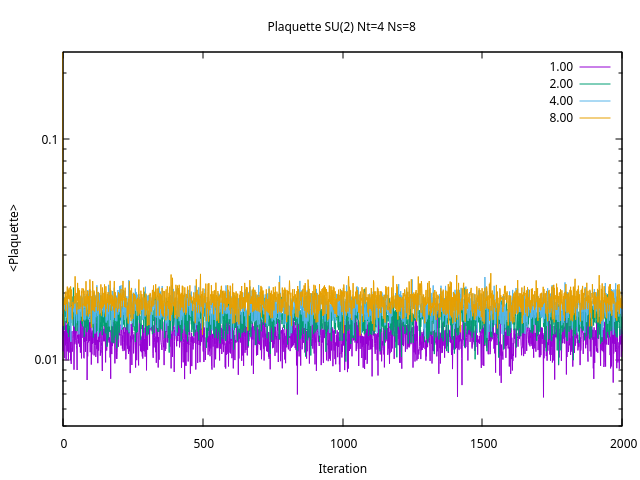
\includegraphics[width=\textwidth]{plaquetteSmallBCT.png}
        \caption{Lattice with $n_t=4$, $n_s=8$.}
        \label{4F:PlaqIterSmallBCT}
    \end{subfigure}
    \begin{subfigure}[b]{0.49\textwidth}
        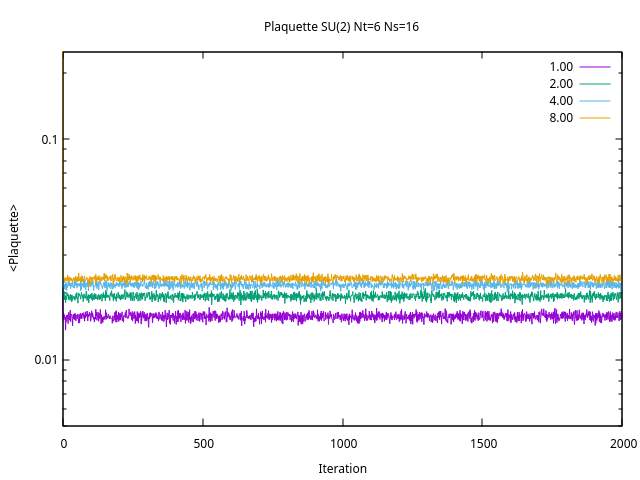
\includegraphics[width=\textwidth]{plaquetteBigBCT.png}
        \caption{Lattice with $n_t=6$, $n_s=16$.}
        \label{4F:PlaqIterBigBCT}
    \end{subfigure}
    \caption{Average value of the triangular plaquette on BCT lattices as a function of the number of iterations. The different colors represent different values of $\beta$.}
    \label{4F:PlaqIterBCT}
\end{figure}\\
In both figures it is clear that the plaquette thermalizes very quickly (only the first few values are significantly different from the others); this is expected, since, like on the hypercubic lattice, the plaquette is a very local quantity, which can be efficiently sampled by the local updates used in the code.
One can also observe that the results from the lattice with most sites have the smallest statistical fluctuations: an effect due to volume averaging.\\
The same simulation has been run on a SH lattice, computing the mean value of the rectangular plaquette \eqref{2:LatticePlaquette}, in order to make a comparison.\\
Results are shown in \figref{4F:PlaqIterSH}.
\begin{figure}[!htbp]
    \centering
    \begin{subfigure}[b]{0.49\textwidth}
        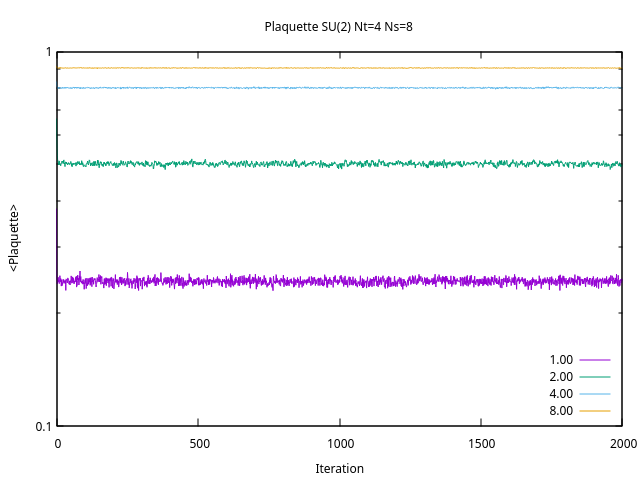
\includegraphics[width=\textwidth]{plaquetteSmallSH.png}
        \caption{Lattice with $n_t=4$, $n_s=8$.}
        \label{4F:PlaqIterSmallSH}
    \end{subfigure}
    \begin{subfigure}[b]{0.49\textwidth}
        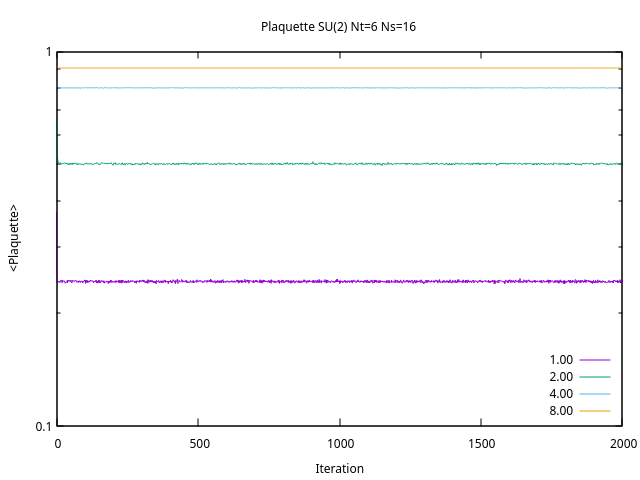
\includegraphics[width=\textwidth]{plaquetteBigSH.png}
        \caption{Lattice with $n_t=6$, $n_s=16$.}
        \label{4F:PlaqIterBigSH}
    \end{subfigure}
    \caption{Average value of the rectangular plaquette on SH lattices as a function of the number of iterations. The different colors represent different values of $\beta$.}
    \label{4F:PlaqIterSH}
\end{figure}\\
Here it can be seen that mean values of the plaquette are more distant from each other than in the BCT case.
They also have smaller fluctuations, albeit the fact that they get smaller by increasing the number of sites of the lattice is observed in both the SH and BCT cases.

\subsubsection{Plaquette Mean Value vs $\beta$}
The mean value of each dataset of \figref{4F:PlaqIterBCT} has also been computed, with the aim of studying the behaviour of the average plaquette with respect to $\beta$.
In the computation of the means, only the last $1000$ values have been taken into account, in order to discard unthermalized values.
\begin{figure}[!htbp]
    \centering
    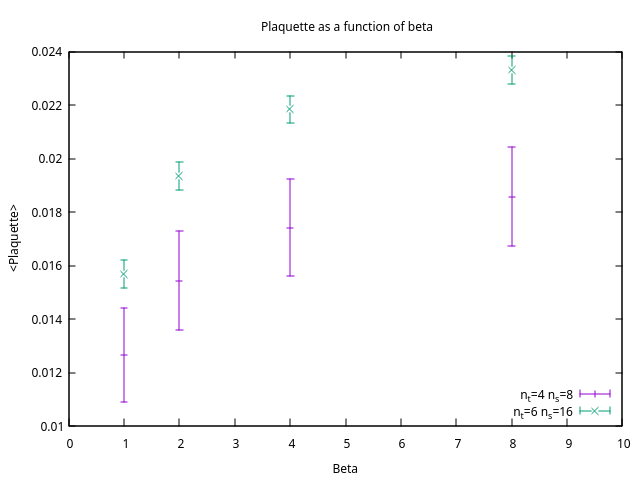
\includegraphics[width=0.5\textwidth]{PlaquetteBetaBCT.png}
    \caption{Mean value of the triangular plaquette on BCT lattices as a function of $\beta$. The purple data is from the smaller lattice ($n_t=4$, $n_s=8$), the green one is from the bigger lattice ($n_t=6$, $n_s=16$).}
    \label{4F:PlaqBetaBCT}
\end{figure}\\
As anticipated, statistical fluctuations of the lattice with a larger number of sites are smaller, thus the statistical uncertainties are smaller than error bars of points obtained from datasets of the lattice with fewer points.\\
\figref{4F:PlaqBetaBCT} reveals that, for these simulations, the plaquette mean values from lattices of different size are not compatible with each other for the same value of $\beta$, and that the dependence on $\beta$ appears not to be compatible with continuum-scaling behavior yet. For this reason, the data cannot be directly compared with \figref{3F:AvgPlaqBCTSH}, which was independently obtained with a different algorithm (and including some different normalizations, too). In fact, it is worth emphasizing that (assuming that there are no bugs in the code) it is only in the continuum limit that the results obtained from different lattice simulations should converge to the same limit.\\
As a side remark, one should also consider that, while the Monte~Carlo history of the average plaquette does not reveal exceedingly long autocorrelation times, some autocorrelation may still be present in the sample of configurations used for this preliminary analysis; in order to study this possibility in a more systematic way, one should carry out a careful analysis of other observables, too -- including, in particular, those that are of non-local nature, since typically they are most severely affected by autocorrelation problems. A typical example could be the topological charge, which (in simulations on standard hypercubic lattices) is notorious for its dramatically long autocorrelation times on fine lattices~\cite{Schaefer:2010hu}. While a systematic study of this quantity could potentially yield further motivation to carry out simulations on a BCT lattice (where better recovery of rotational symmetry can be achieved at coarser lattice spacings), this is clearly beyond the scope of the present M.Sc. thesis work, and we leave it for a dedicated future project~\cite{Aliberti:2024soa}.
%Although the first problem could be ``circumvented'' by considering the autocorrelation of the data, thus increasing the error bars, the second one has not a simple explanation and leads to think that there could be a possible bug in the code.\\
%Again, in order to make a comparison, the same plot has been reproduced for the SH lattice, using the last $1000$ data from each dataset of \figref{4F:PlaqIterBCT}.\\
%Results are shown in \figref{4F:PlaqBetaSH}.
%\begin{figure}[!htbp]
%    \centering
%    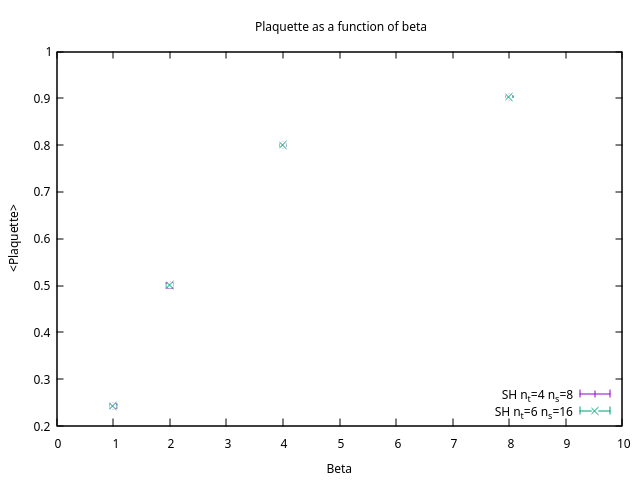
\includegraphics[width=0.5\textwidth]{PlaquetteBetaSH.png}
%    \caption{Mean value of the rectangular plaquette on SH lattices as a function of $\beta$. The purple data is from the smaller lattice ($n_t=4$, $n_s=8$), the green one is from the bigger lattice ($n_t=6$, $n_s=16$).}
%    \label{4F:PlaqBetaSH}
%\end{figure}
%This plot makes even more evident the problems mentioned before: in SH lattices, error bars are orders of magnitude smaller than those of BCT lattices and the average value of the plaquettes does not evidently depend on the size of the lattice.
%Furthermore, increasing $\beta$ (therefore decreasing the coupling constant $g$, \ie weakening the interaction) makes the averages tend to $1$, much more than the data obtained from BCT lattices and a lot more in accordance with \figref{3F:AvgPlaqBCTSH}.\\
%This is probably due to an error in the code, that needs to be investigated further.


\newpage
\cleardoublepage
\pagestyle{myFancy}
\chapter{Conclusions}

In this M.Sc. thesis work, we addressed the problem of the restoration of the correct space-time symmetries in the continuum limit of lattice field theory.
Given the paramount relevance of space-time symmetries in quantum field theory, the correct restoration of such symmetries when the lattice spacing $a$ is sent to zero is a very important requirement, in order to obtain the correct physics from lattice calculations.

Unlike translational invariance, that on a regular lattice is broken down to translations by integer multiples of the lattice spacing $a$ (so that continuous translations are naively recovered in the $a \to 0$ limit), rotational invariance is broken down to a discrete subgroup that \emph{does not} depend on $a$, but only on the geometry of the lattice, making the effective restoration of rotational invariance in the continuum limit non-trivial.

Indeed, the symmetry-breaking terms of rotational invariance are expected to be suppressed by some positive powers of the lattice spacing in the $a\to 0$ limit, but the nature of these symmetry-breaking terms, as well as the form and magnitude of their coefficients, depend on the lattice chosen for the discretization of the space-time.

For this reason, in the present M.Sc. thesis we compared the lattice discretization of four-dimensional Euclidean space based on a hypercubic lattice, with one based on the lattice of roots of the Lie algebra of the generators of the exceptional simple Lie group $\spF$, which features more vectors and is the most symmetric regular lattice existing in four dimensions.
This type of lattice is also known as Body-Centered Tesseract (BCT).

To monitor the restoration of rotational symmetry at the non-perturbative level, which is particularly important for quantum chromodynamics and for other strongly coupled non-Abelian gauge theories, we studied the expectation value of some quantities that are expected to be rotationally invariant in the continuum theory, like the static quark potential.
In particular, as we discussed in \secref{Sec4:RotInv}, we focused on the rotational symmetry restoration for the potential associated to a pair of static color sources in (purely gluonic) $\SU(2)$ Yang-Mills theory.

Regularizing QCD on a lattice with higher symmetry than the usual hypercubic one could allow the restoration of the rotational symmetry of the various physical quantities on lattices with a coarser spacing.
This would potentially have obvious advantages in terms of computational costs (for a fixed physical hypervolume, the number of degrees of freedom of the lattice theory scales like the fourth power of the inverse lattice spacing), in particular in view of the severe autocorrelation times that affect topological quantities in lattice QCD simulations carried out on fine hypercubic lattices.

After creating the original code presented in \secref{Sec4:Code} we carried out a preliminary study of the simulation of $\SUN$ Yang-Mills theories on the BCT lattice.
In principle, our code could be easily extended to simulate the theory also on the \spFtext coroots lattice, which would correspond to include additional ``improvement terms'' in the lattice action, and could lead to an even more rapid restoration of the continuum symmetries.
This gain may offset and possibly overcompensate for the increased computational costs due to the extra terms required in the update of lattice field configurations on a Euclidean grid with this type of geometry.

Our numerical study, however, was limited to the BCT lattice; it included the definition of an action, different from the Wilson action used in hypercubic lattice simulations, in terms of the smallest triangular plaquettes that can be defined on the BCT.

The simulations of $\SU(2)$ Yang-Mills theory on a BCT lattice that we carried out showed a quick thermalization of the mean value of the plaquette and the reduction of the magnitude of statistical fluctuations as the hypervolume is increased.
Both these effects were expected, the first one because of the locality of the observable, the second one because of the volume averaging effect.
This is a sign that the algorithm is well-behaving, at least under these aspects.

Plots of the plaquette mean values as functions of the parameter $\beta$ (which is inversely proportional to the square of the bare coupling of the lattice theory $g$), on the other hand, showed that mean values obtained from simulations on lattices of different size were not fully compatible with each other: assuming that these results were not due to some subtle bug in the code (our code successfully passed all the main tests, including those related to gauge invariance of the results, etc., but this would not rule out the existence of some non-trivial undesired artifact in our numerical implementation of the lattice theory) this could mean that, with the action used, these values of $\beta$ are not yet close to the continuum limit.
Alternatively, these effects may be indeed due to some actual ``physical'' property of this lattice theory: examples include the possible existence of so far unknown transition lines or crossover lines in the phase diagram having as axes the bare coupling of the lattice theory and the system sizes. As a matter of fact, a precise exploration of the phase diagram of this lattice theory and the location of points where continuous transitions exist remains an important task for future studies; indeed, observables from different simulations should converge to the same limit only while approaching the continuum, which means approaching a point in the phase diagram of the theory where the correlation length in units of the lattice spacing is divergent.

To conclude, we remark that the work carried out in this M.Sc. thesis also sets the basis for future studies on this subject, in particular the systematic study of quantities with longer autocorrelation times than the plaquette, like the topological charge, could yield better results than those that at present can be obtained from simulations on the hypercubic lattice. A complete study of this problem will be presented elsewhere~\cite{Aliberti:2024soa}.

Another interesting study could be a dedicated and detailed evaluation of the static quark potential, that has already been studied extensively on the hypercubic lattice, in order to check if the recovery of rotational invariance occurs at larger lattice spacings, and to quantify the gain in terms of computing time.

Finally, given that QCD also includes quarks, beside gluons, in the future it would also be interesting to study the discretization of fermions on this highly symmetric lattice.


\newpage
\cleardoublepage
\appendix
\pagenumbering{Roman}

\newpage
\cleardoublepage
\pagestyle{myFancy}
\chapter{Code}

File \texttt{initialize.cc}:
\lstinputlisting[lastline=9]{initialize.cc}
\lstinputlisting[firstline=117, lastline=136, firstnumber=117]{initialize.cc}
\lstinputlisting[firstline=160, lastline=257, firstnumber=160]{initialize.cc}
\lstinputlisting[firstline=258, lastline=308, firstnumber=258]{initialize.cc}
\lstinputlisting[firstline=309, lastline=360, firstnumber=309]{initialize.cc}
\lstinputlisting[firstline=361, lastline=412, firstnumber=361]{initialize.cc}
\lstinputlisting[firstline=413, lastline=464, firstnumber=413]{initialize.cc}
\lstinputlisting[firstline=465, lastline=516, firstnumber=465]{initialize.cc}
\lstinputlisting[firstline=517, lastline=523, firstnumber=517]{initialize.cc}
\lstinputlisting[firstline=668, lastline=672, firstnumber=668]{initialize.cc}
\lstinputlisting[firstline=677, lastline=694, firstnumber=677]{initialize.cc}
\lstinputlisting[firstline=743, lastline=749, firstnumber=743]{initialize.cc}
\lstinputlisting[firstline=758, lastline=764, firstnumber=758]{initialize.cc}
\lstinputlisting[firstline=773, lastline=779, firstnumber=773]{initialize.cc}
\lstinputlisting[firstline=788, lastline=794, firstnumber=788]{initialize.cc}
\lstinputlisting[firstline=758, lastline=764, firstnumber=758]{initialize.cc}
\lstinputlisting[firstline=803, lastline=809, firstnumber=803]{initialize.cc}
\lstinputlisting[firstline=818, lastline=824, firstnumber=818]{initialize.cc}
\lstinputlisting[firstline=833, lastline=839, firstnumber=833]{initialize.cc}
\lstinputlisting[firstline=848, lastline=854, firstnumber=848]{initialize.cc}
\lstinputlisting[firstline=863, lastline=869, firstnumber=863]{initialize.cc}
\lstinputlisting[firstline=878, lastline=884, firstnumber=878]{initialize.cc}
\lstinputlisting[firstline=893, lastline=899, firstnumber=893]{initialize.cc}
\lstinputlisting[firstline=908, lastline=914, firstnumber=908]{initialize.cc}
\lstinputlisting[firstline=923, lastline=924, firstnumber=923]{initialize.cc}
\lstinputlisting[firstline=1059, lastline=1063, firstnumber=1059]{initialize.cc}
\lstinputlisting[firstline=1141, lastline=1142, firstnumber=1141]{initialize.cc}
\newpage

File \texttt{f4pstaple.cc}:
\lstinputlisting{f4pstaple.cc}
\newpage

File \texttt{f4nstaple.cc}:
\lstinputlisting{f4nstaple.cc}
\newpage

File \texttt{plaquette.cc}:
\lstinputlisting[lastline=4]{plaquette.cc}
\lstinputlisting[firstline=11, lastline=11, firstnumber=11]{plaquette.cc}
\lstinputlisting[firstline=15, lastline=15, firstnumber=15]{plaquette.cc}
\lstinputlisting[firstline=17, lastline=17, firstnumber=17]{plaquette.cc}
\lstinputlisting[firstline=21, lastline=21, firstnumber=21]{plaquette.cc}
\lstinputlisting[firstline=23, lastline=45, firstnumber=23]{plaquette.cc}
\lstinputlisting[firstline=68, lastline=74, firstnumber=68]{plaquette.cc}


\newpage
\cleardoublepage
\pagestyle{solopagina}
\printbibliography


\newpage
\cleardoublepage
\pagestyle{solopagina}
\renewcommand{\headrulewidth}{0.0pt}
\fancyhead{}
\fancyfoot{}

\section*{Acknowledgements}

Giunto alla fine di questo lungo viaggio, desidero ringraziare tutte le persone che mi hanno supportato.

Primo fra tutti il mio relatore, Marco Panero, per tutti i preziosi consigli e le correzioni, senza i quali questo lavoro di tesi non sarebbe riuscito così bene.

Poi, tutti i miei docenti delle scuole secondarie inferiori e superiori, per aver fatto nascere e coltivato in me la passione per lo studio e per questa bellissima materia e per aver ampliato e fatto crescere il mio bagaglio culturale, facendo sì che non si limitasse a poche discipline.

Un ringraziamento speciale va ai miei compagni di corso, che non sono stati solo dei \emph{compagni di viaggio}, ma delle persone con le quali ho condiviso gioie, sofferenze e importanti momenti di confronto tra una lezione e l'altra, che hanno contribuito ad accrescere le mie conoscenze approfondendo gli argomenti trattati nei corsi.

Desidero ringraziare anche tutti i miei amici e parenti più stretti per avermi supportato (sia economicamente che emotivamente) e per essermi stati accanto anche nei momenti più difficili, in particolare i miei genitori, mio fratello, i miei nonni e Francesca, che è la persona migliore che abbia mai conosciuto e che ha creduto in me più di quanto io non abbia fatto con me stesso.

Infine, un grazie a tutti quelli che sono riusciti a ritagliarsi una parte del loro tempo per essere qui con me alla discussione e anche a tutti quelli che non hanno potuto farlo, ma che sono con me con il pensiero.


\end{document}
